
\section{List of triggers used in the analysis}
\label{app:trigger_list}
\hspace{10pt} Table~\ref{a_tab:triggers} shows the list of HLT algorithms used in the analysis. The corresponding input L1 seeds are listed for each HLT path, with the separation being made for each era of data taking in order to present different thresholds for each year.

\begin{sidewaystable}

    \centering
    \def\arraystretch{1.5}

    \small
    \caption{List of HLT paths accompanied by corresponding L1 seeds used as input~\cite{note:AN_19_257}.
    During the 2017 era the L1\_DoubleJet seeds imposed thresholds for leading jet $p_T$ threshold ranging from 90 to 115~GeV, while the subleading jet threshold took values from 30 to 40~GeV.
    Similarely for the 2018 era, the L1\_DoubleJet seeds required the leading jet $p_T$ threshold range from 90 to 120~GeV and the subleading jet $p_T$ minimum value ranging from 30 to 45~GeV.}

    \footnotesize
    \begin{tabular}{l l c c}
        \hline\hline
        Year                   & HLT path                                                  & L1 seed                         & Primary dataset               \\\hline\hline
        \multirow{5}{*}{2017}  & HLT\_PFMETNoMu120\_PFMHTNoMu120\_IDTight                  & \texttt{L1\_ETMHF70}            & MET                           \\
                               & HLT\_PFMETNoMu120\_PFMHTNoMu120\_IDTight\_PFHT60          & \texttt{L1\_ETMHF80\_HTT60er }  & MET                           \\\cline{2-4}
                               & HLT\_Ele35\_WPTight\_Gsf                                  & \texttt{L1\_SingleEG24}         & SingleElectron                \\\cline{2-4}
                               & \multirow{3}{*}{HLT\_Photon200}                           & \texttt{L1\_SingleEG30}         & \multirow{3}{*}{SinglePhoton} \\
                               &                                                           & \texttt{L1\_SingleJet170}       &                               \\
                               &                                                           & \texttt{L1\_SingleTau100er2p1}  &                               \\\cline{2-4}
                               & HLT\_DiJet110\_35\_Mjj650\_PFMET110                       & \texttt{L1\_DoubleJet\_*\_*\_DoubleJet*\_Mass\_Min620}       &        \\\cline{2-4}
                               & HLT\_TripleJet110\_35\_35\_Mjj650\_PFMET110               & \texttt{L1\_DoubleJet\_*\_*\_DoubleJet*\_Mass\_Min620}       &
                               \\\hline\hline

        \multirow{11}{*}{2018} & \multirow{2}{*}{HLT\_PFMETNoMu120\_PFMHTNoMu120\_IDTight} & \texttt{L1\_ETMHF100}           & \multirow{3}{*}{MET}          \\
                               &                                                           & \texttt{L1\_ETM150}             &                               \\
                               & HLT\_PFMETNoMu120\_PFMHTNoMu120\_IDTight\_PFHT60          & \texttt{L1\_ETMHF90\_HTT60er}   &                               \\\cline{2-4}
                               & \multirow{3}{*}{HLT\_Ele32\_WPTight\_Gsf}                 & \texttt{L1\_SingleIsoEG24er2p1} & \multirow{3}{*}{EGamma}       \\
                               &                                                           & \texttt{L1\_SingleEG26er2p5}    &                               \\
                               &                                                           & \texttt{L1\_SingleEG60}         &                               \\\cline{2-4}

                               & \multirow{5}{*}{HLT\_Photon200}                           & \texttt{L1\_SingleEG34er2p5}    & \multirow{5}{*}{EGamma}       \\
                               &                                                           & \texttt{L1\_SingleJet160er2p5}  &                               \\
                               &                                                           & \texttt{L1\_SingleJet180}       &                               \\
                               &                                                           & \texttt{L1\_SingleTau120er2p1}  &                               \\
                               &                                                           & \texttt{L1\_SingleEG60}         &                               \\\cline{2-4}
                               & \multirow{2}{*}{HLT\_DiJet110\_35\_Mjj650\_PFMET110}      & \texttt{L1\_DoubleJet\_*\_*\_DoubleJet*\_Mass\_Min620}       &  \\
                               &                                                      & \texttt{L1\_DoubleJet\_*\_*\_DoubleJet*\_Mass\_Min620\_Jet60TT28} &
                               \\\cline{2-4}
                               & \multirow{2}{*}{HLT\_TripleJet110\_35\_35\_Mjj650\_PFMET110} & \texttt{L1\_DoubleJet\_*\_*\_DoubleJet*\_Mass\_Min620} & \\
                               &                                                             & \texttt{L1\_DoubleJet\_*\_*\_DoubleJet*\_Mass\_Min620\_Jet60TT28} & \\\hline


        \hline\hline %--------------------------------------------------------------------------------------------------------------------------      \
    \end{tabular}

    \label{a_tab:triggers}

\end{sidewaystable}

\section{Analysis strategy for the 2018 era}
\label{app:MTR_2018}
\hspace{10pt} Figures~\ref{fig:2018_SR_motivation_1} and~\ref{fig:2018_SR_motivation_2} show the distributions of main analysis variables in the SR after the full MTR selection being applied, for the 2018 era. The corresponding distributions for the VTR category are given in figures~\ref{fig:2018_VTR_SR_motivation_1} and~\ref{fig:2018_VTR_SR_motivation_2}.

\hspace{10pt} Continuing the discussion regarding the problem of jet "horns", Figures~\ref{fig:jet_eta_preHornCut_2018} and~\ref{fig:jet_eta_postHornCut_2018} show distributions of jet $\eta$ for the leading jet pair, pre and post mitigation veto being applied, respectively (for both categories).

\begin{figure}[htbp]
  \centering
      \subfigure[\mindphi]{
    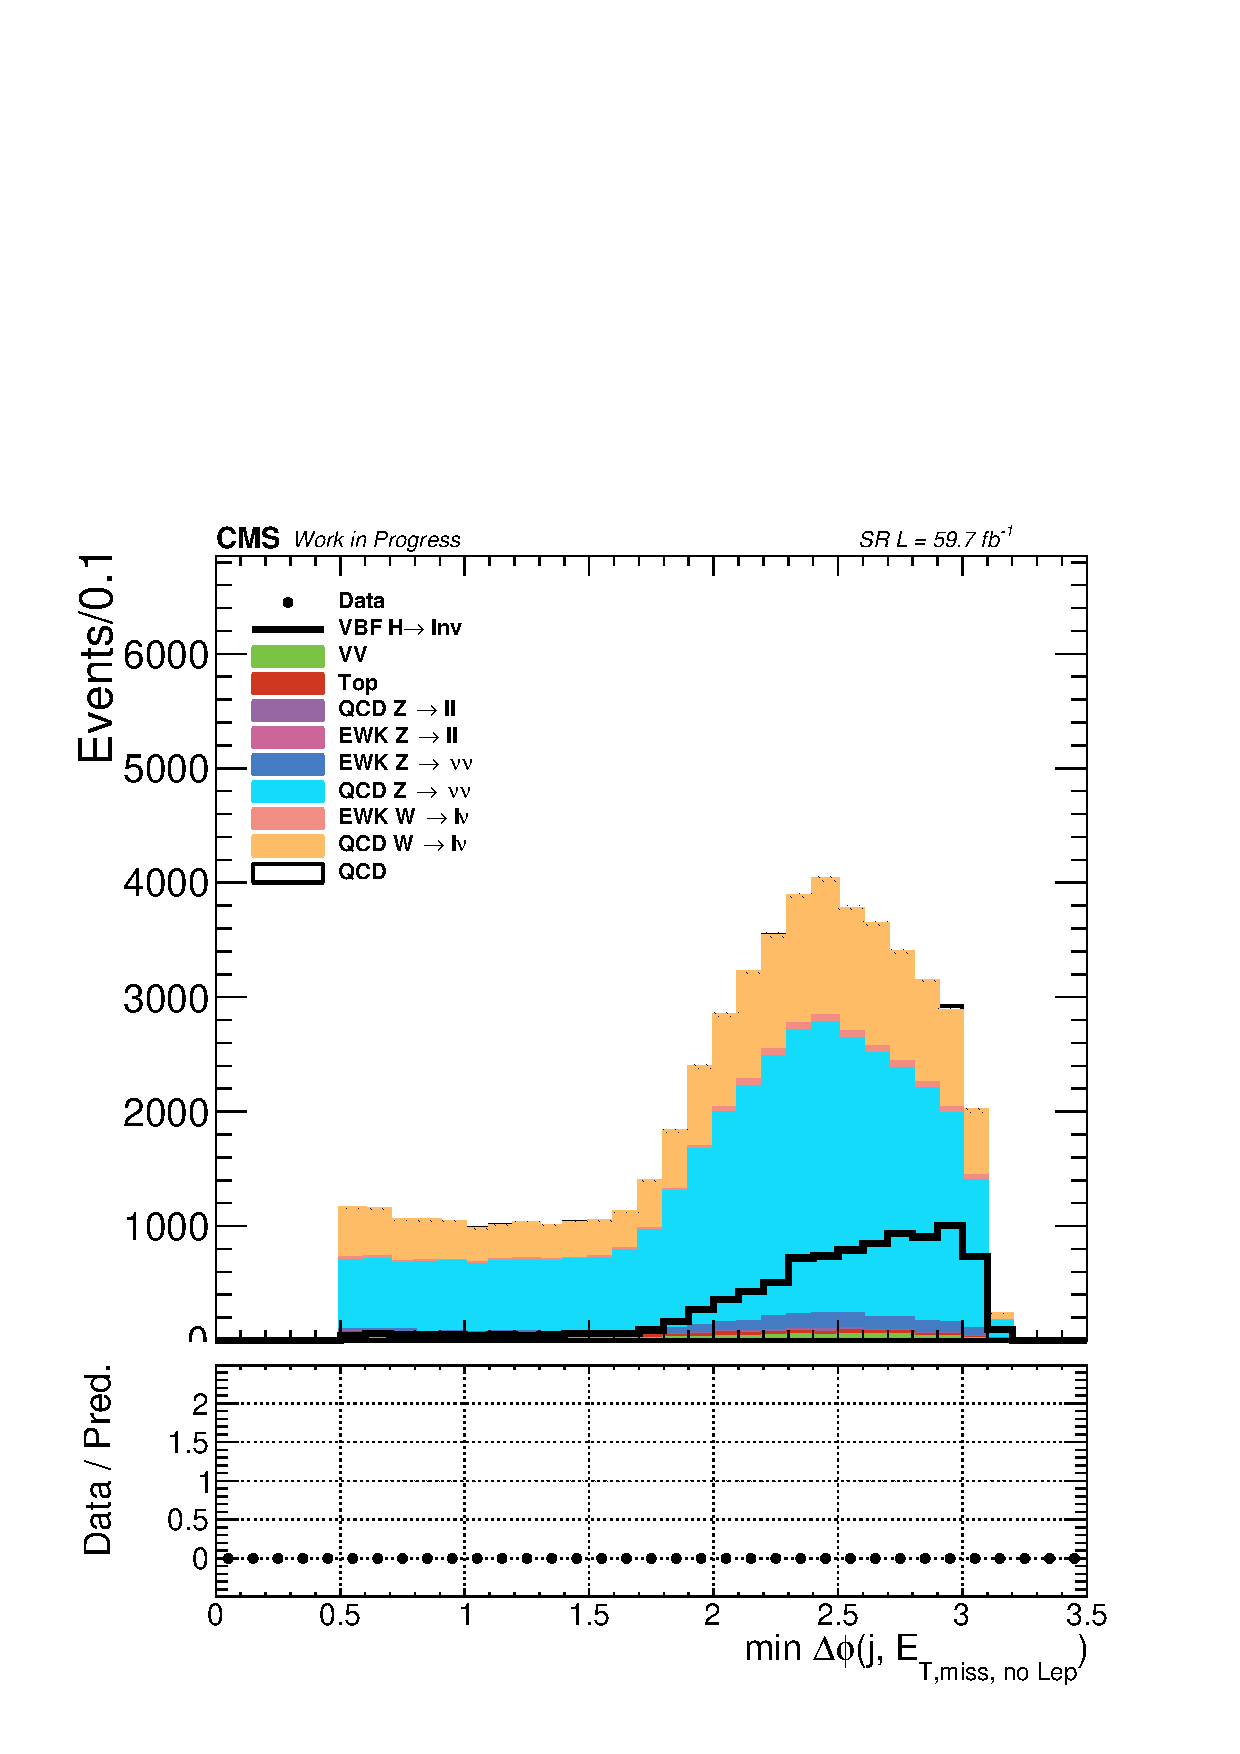
\includegraphics[width=0.49\textwidth]{Analysis_strategy/MTR_2018_SR/MetNoLep_CleanJet_mindPhi.pdf}
    }\\
    \subfigure[$\Delta\eta_{jj}$]{
    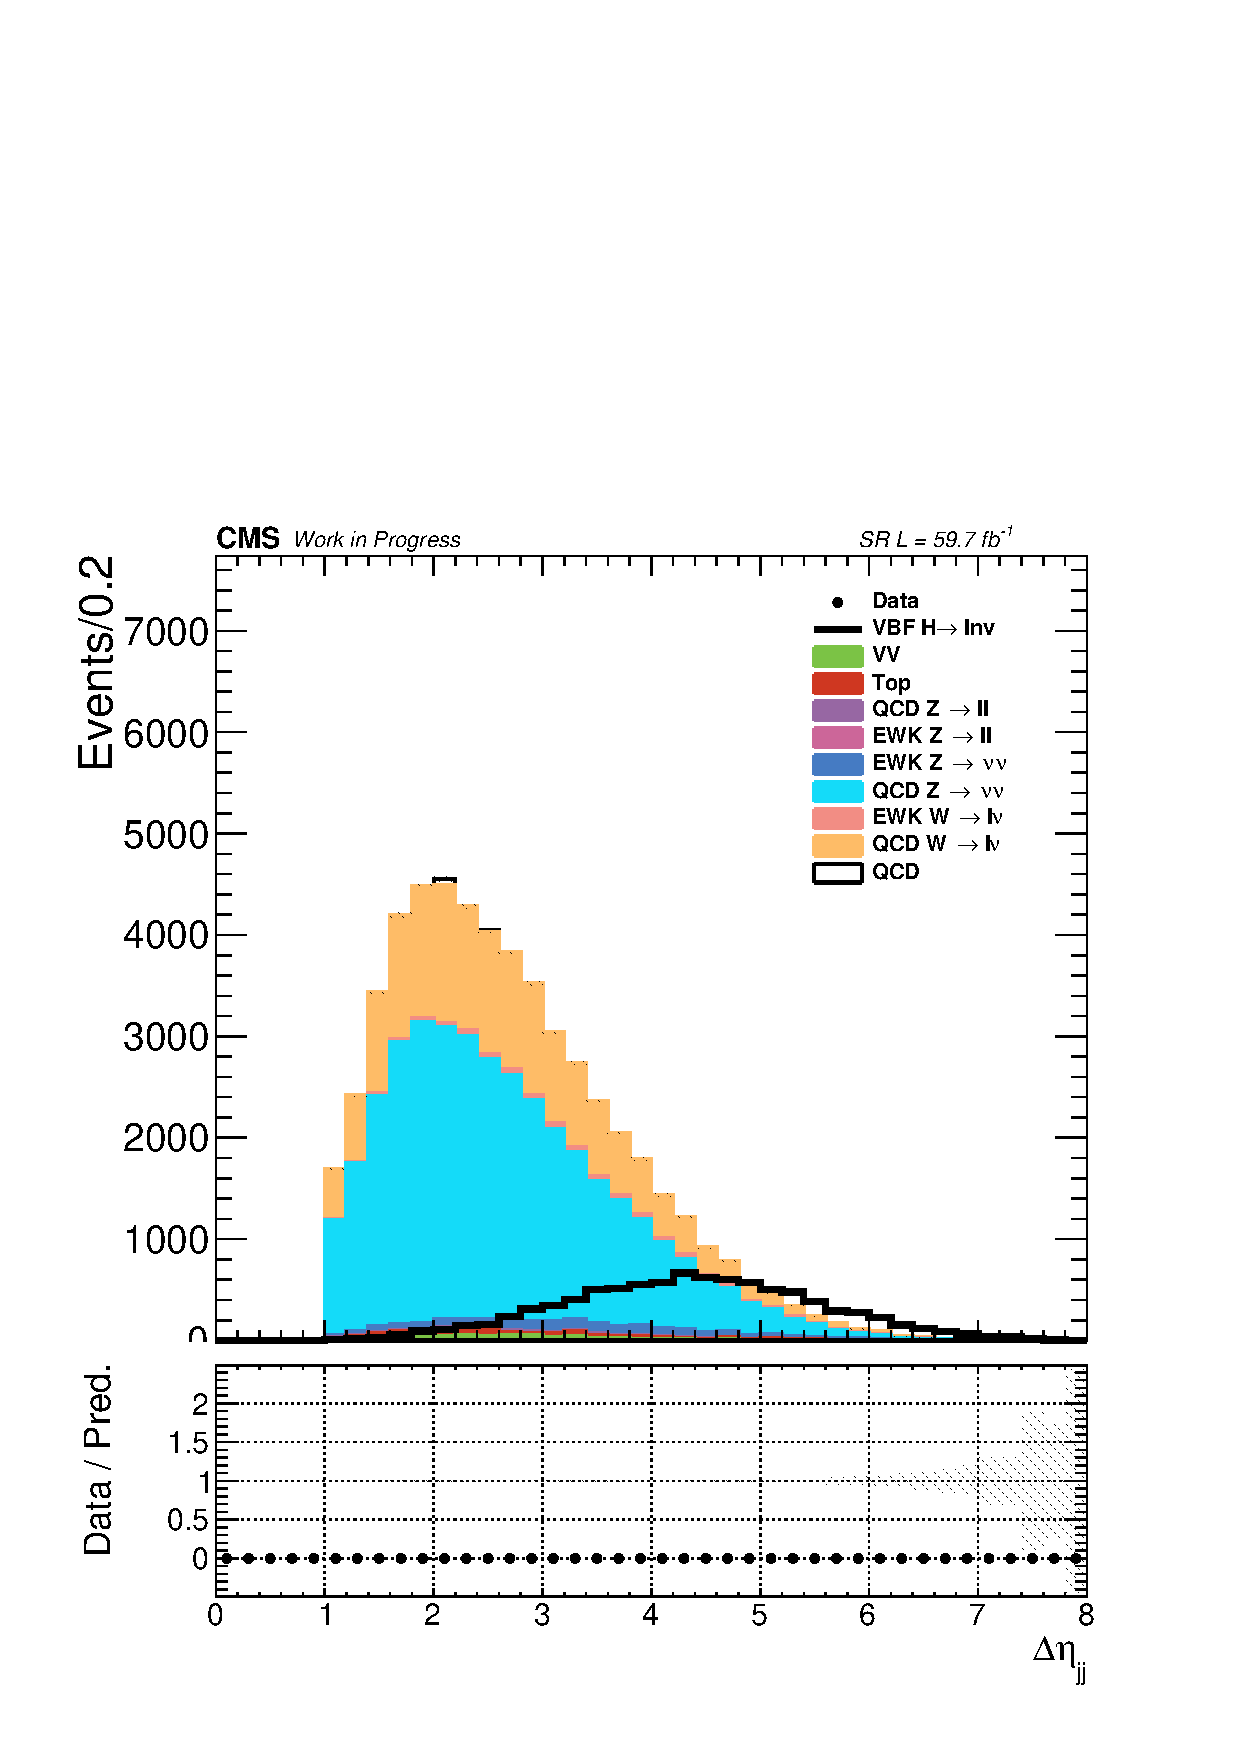
\includegraphics[width=0.49\textwidth]{Analysis_strategy/MTR_2018_SR/leading_dEtajj.pdf}
    }
    \subfigure[$\Delta\phi_{jj}$]{
    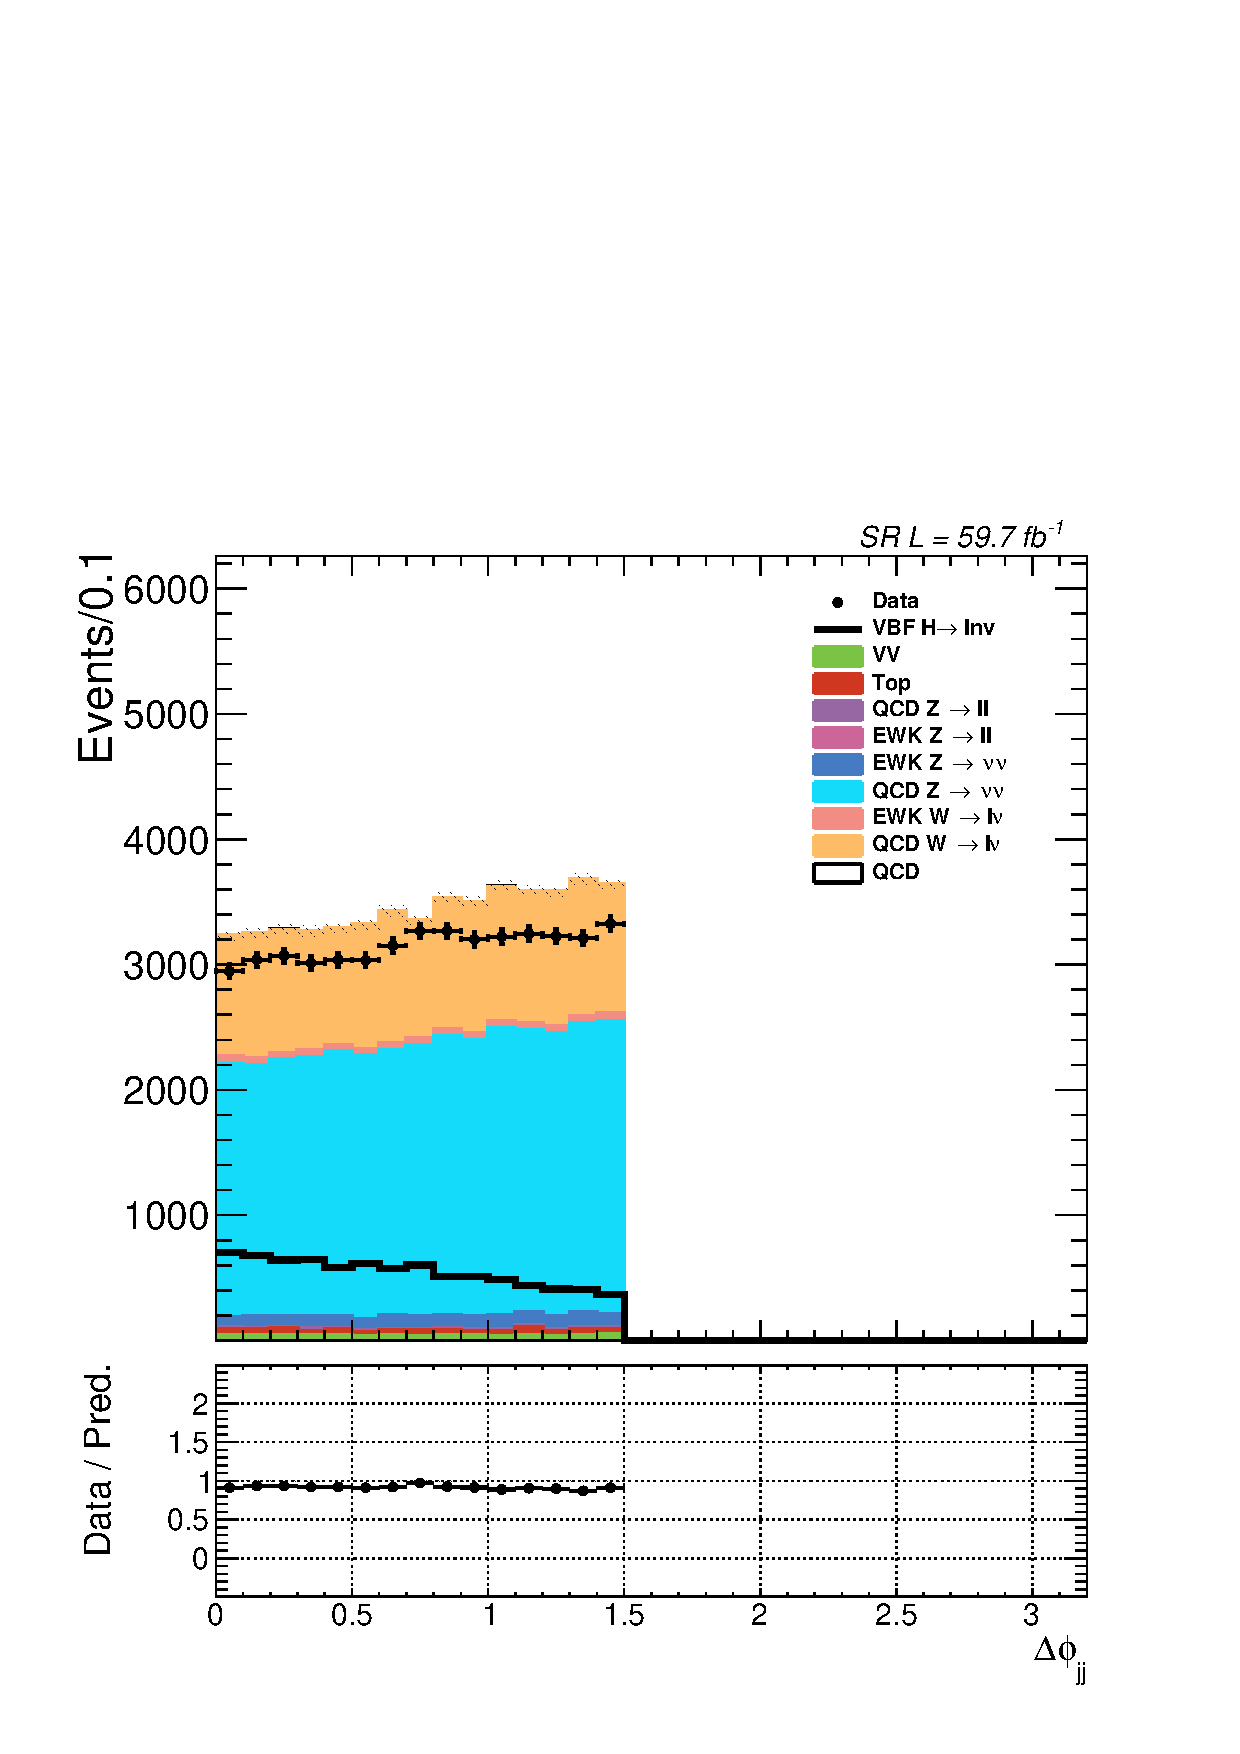
\includegraphics[width=0.49\textwidth]{Analysis_strategy/MTR_2018_SR/leading_dPhijj.pdf}
    }
  \caption{Distributions of \mindphi, $\Delta\eta_{jj}$ and $\Delta\phi_{jj}$ variables in the SR after the full MTR selection, representing the 2018 era.}
  \label{fig:2018_SR_motivation_1}
\end{figure}
\begin{figure}[htbp]
  \centering
      \subfigure[$E_{T,miss}$]{
    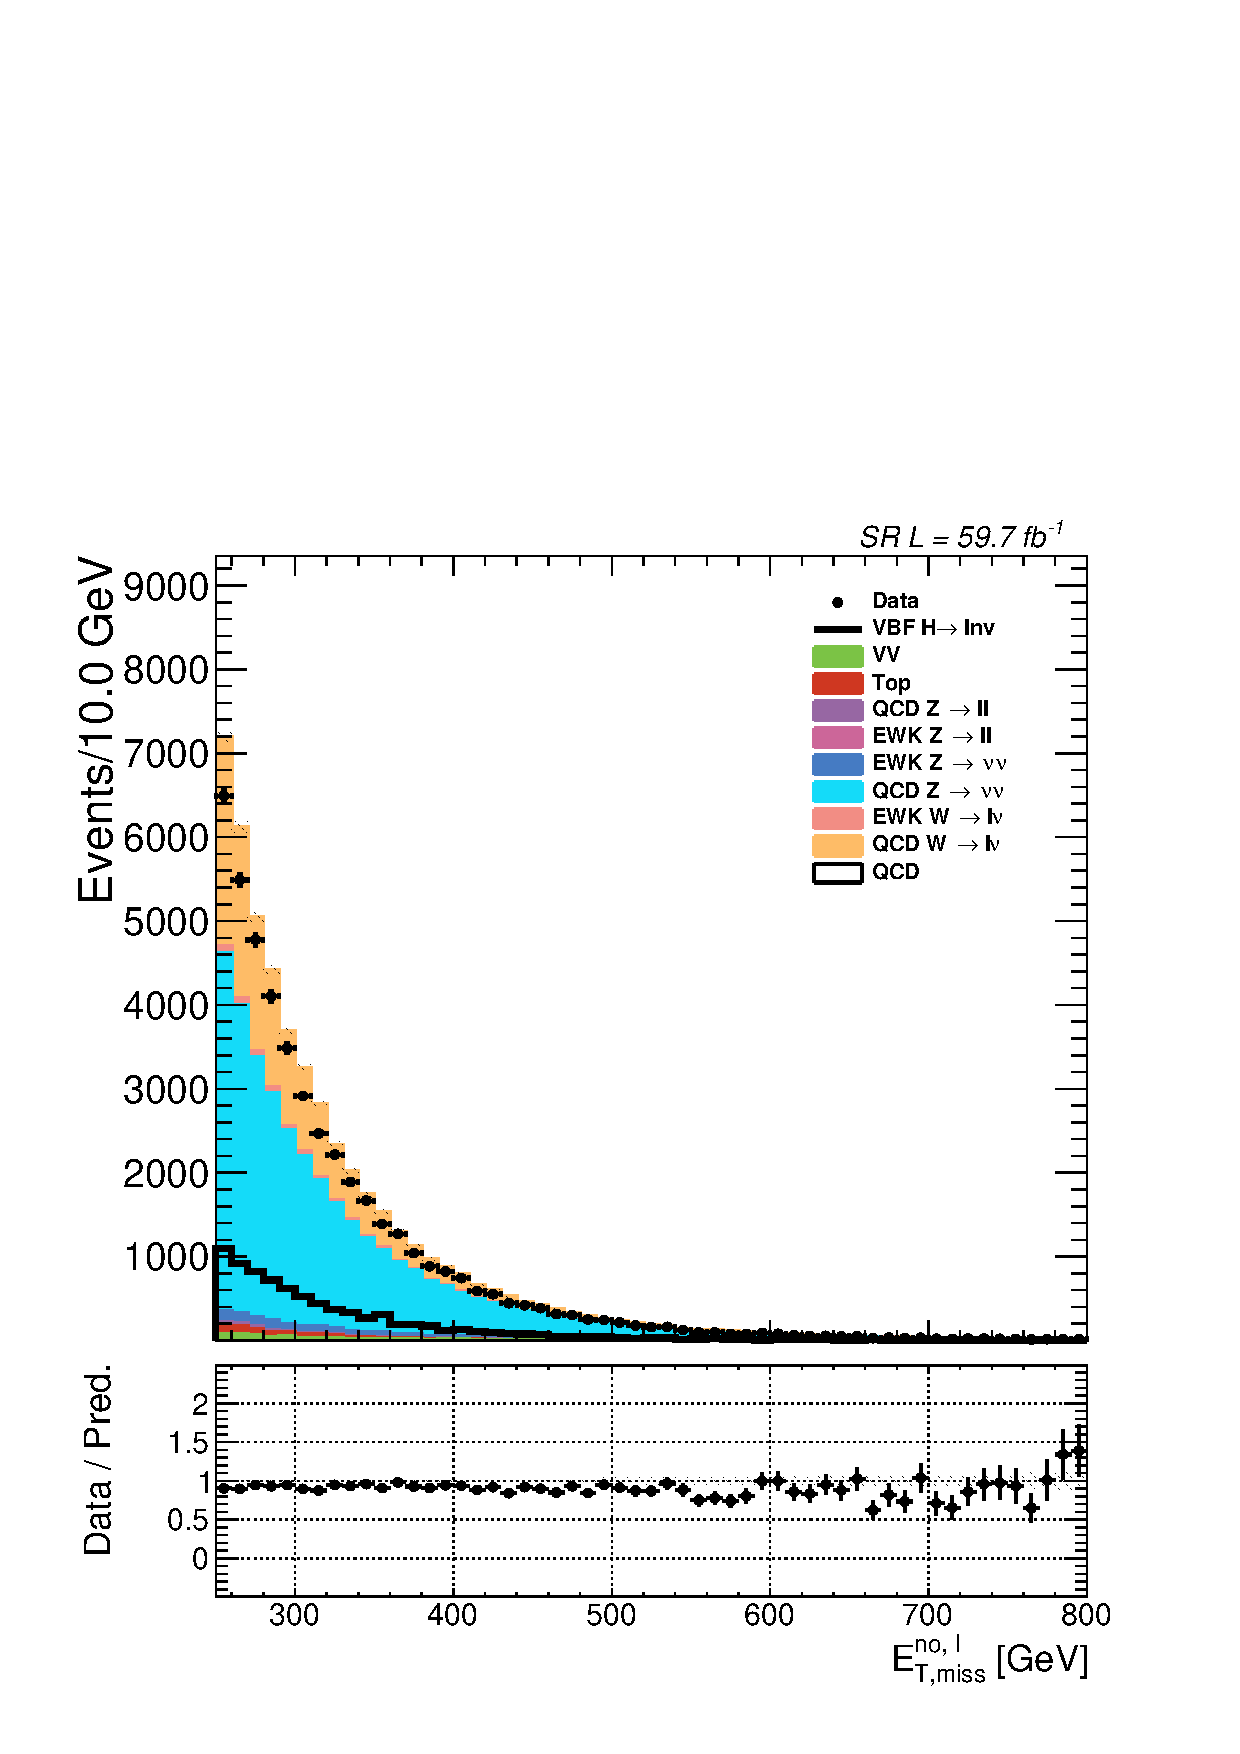
\includegraphics[width=0.49\textwidth]{Analysis_strategy/MTR_2018_SR/MetNoMu.pdf}
    }
    \subfigure[$M_{jj}$]{
    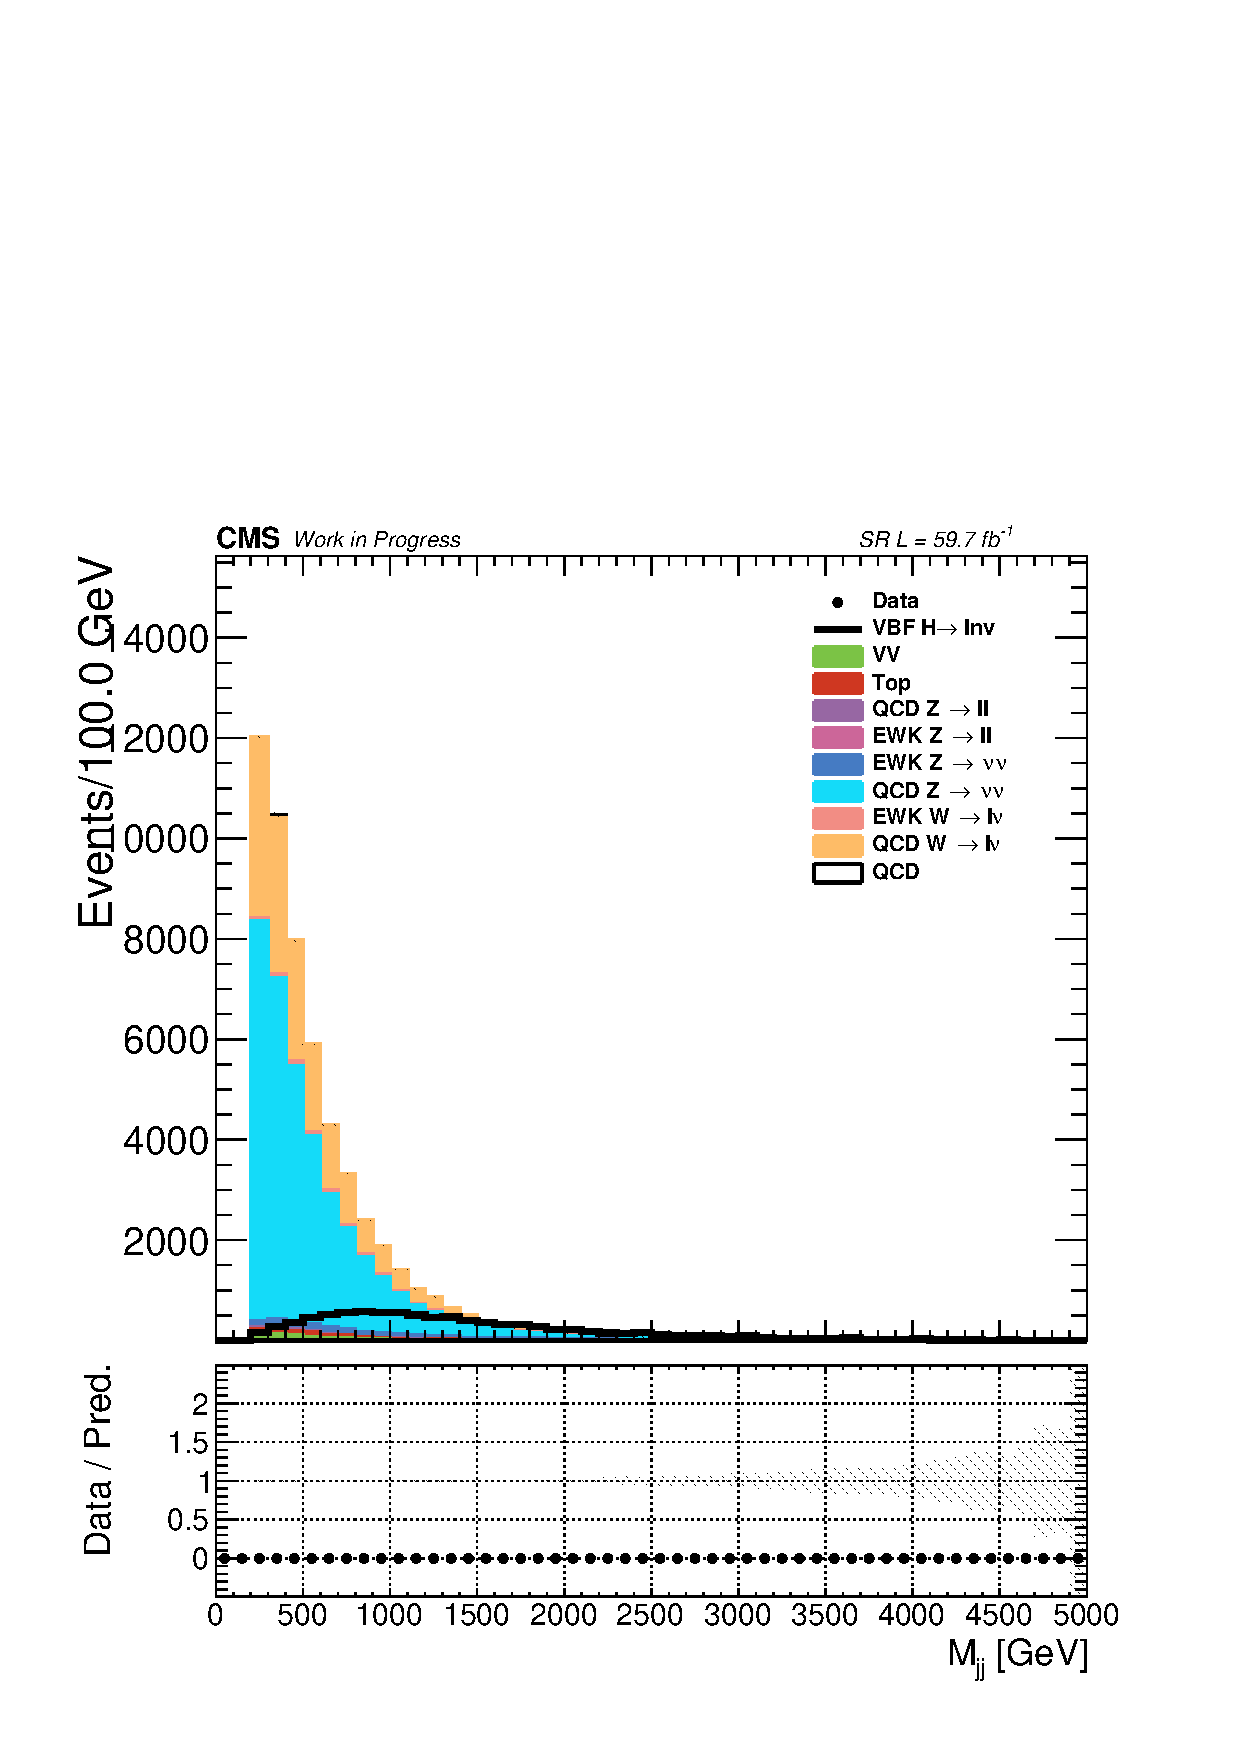
\includegraphics[width=0.49\textwidth]{Analysis_strategy/MTR_2018_SR/leadingJet_mjj.pdf}
    }\\
    \subfigure[$p_{T,j1}$]{
    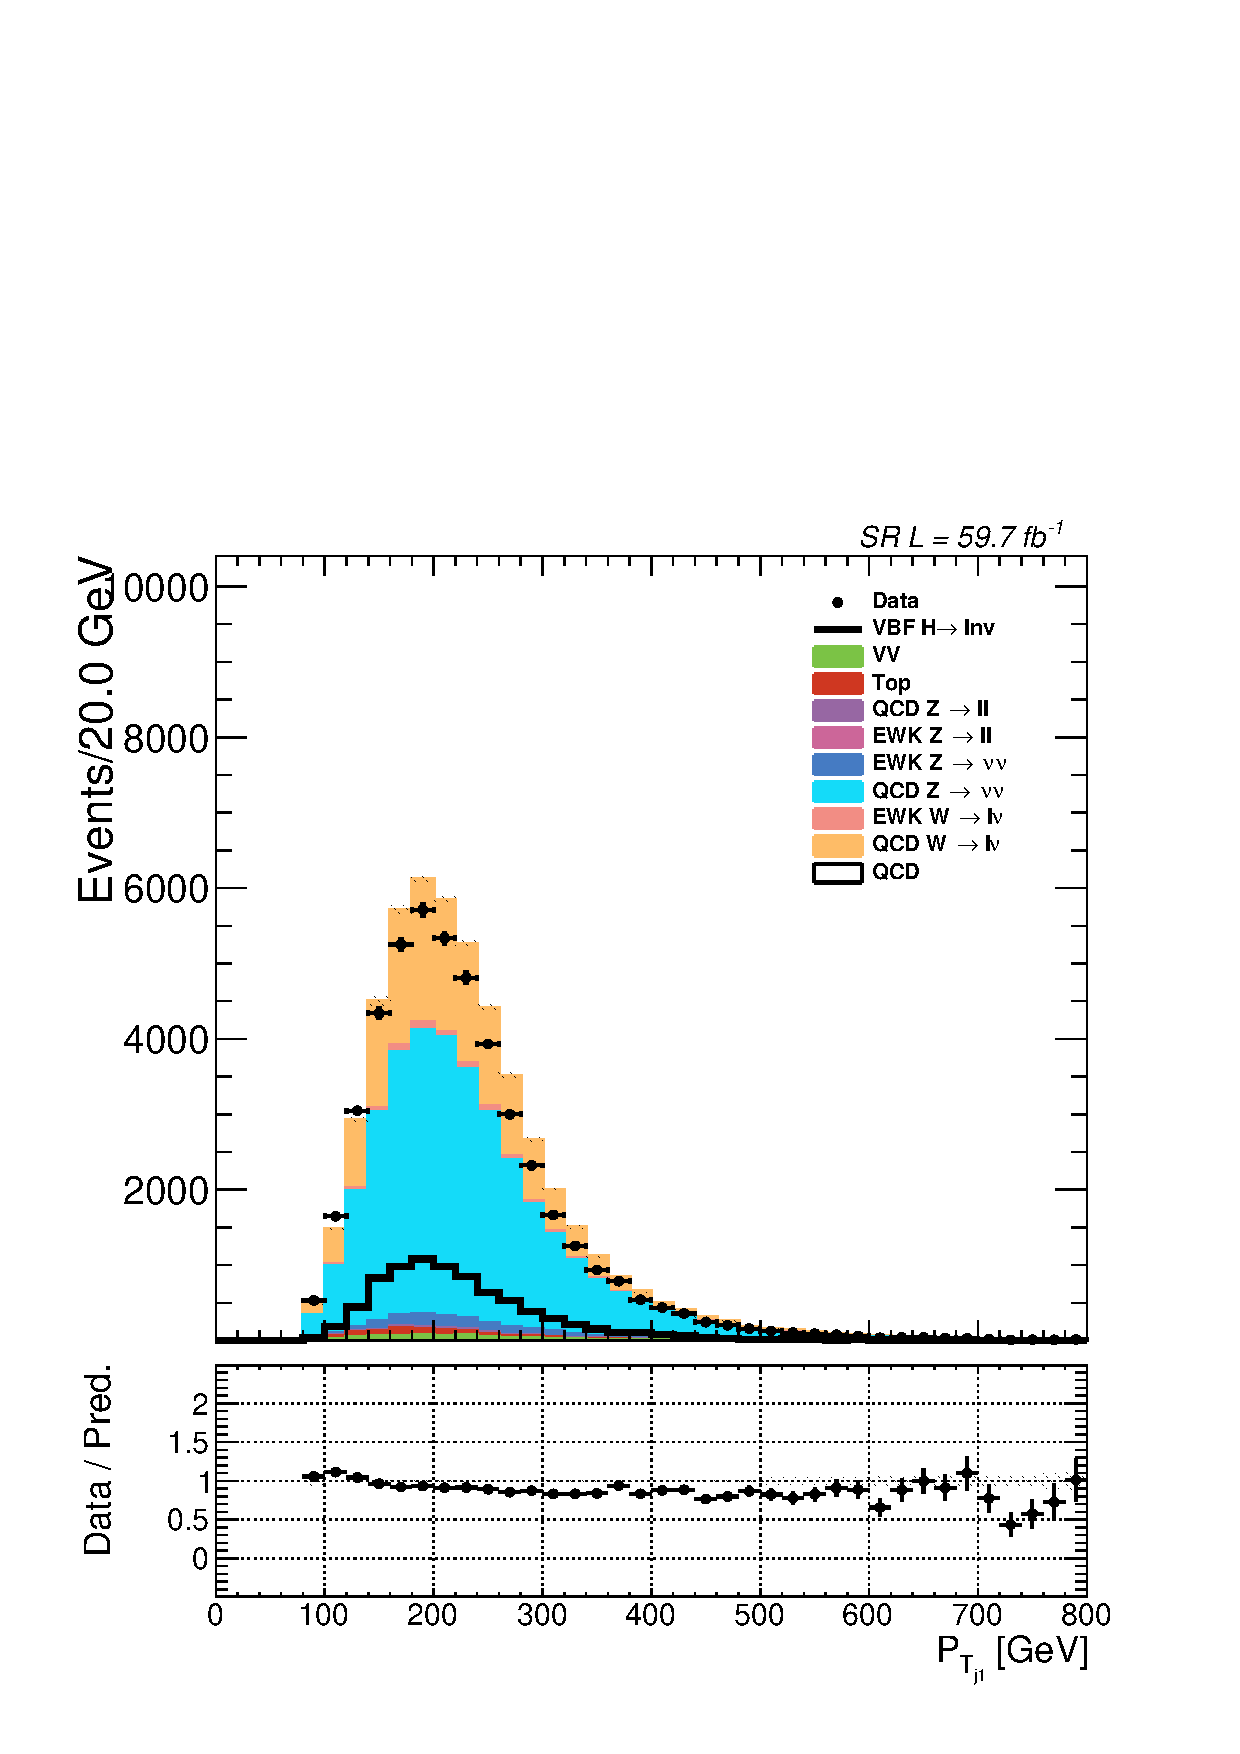
\includegraphics[width=0.49\textwidth]{Analysis_strategy/MTR_2018_SR/Leading_jet_pt.pdf}
    }
    \subfigure[$p_{T,j2}$]{
    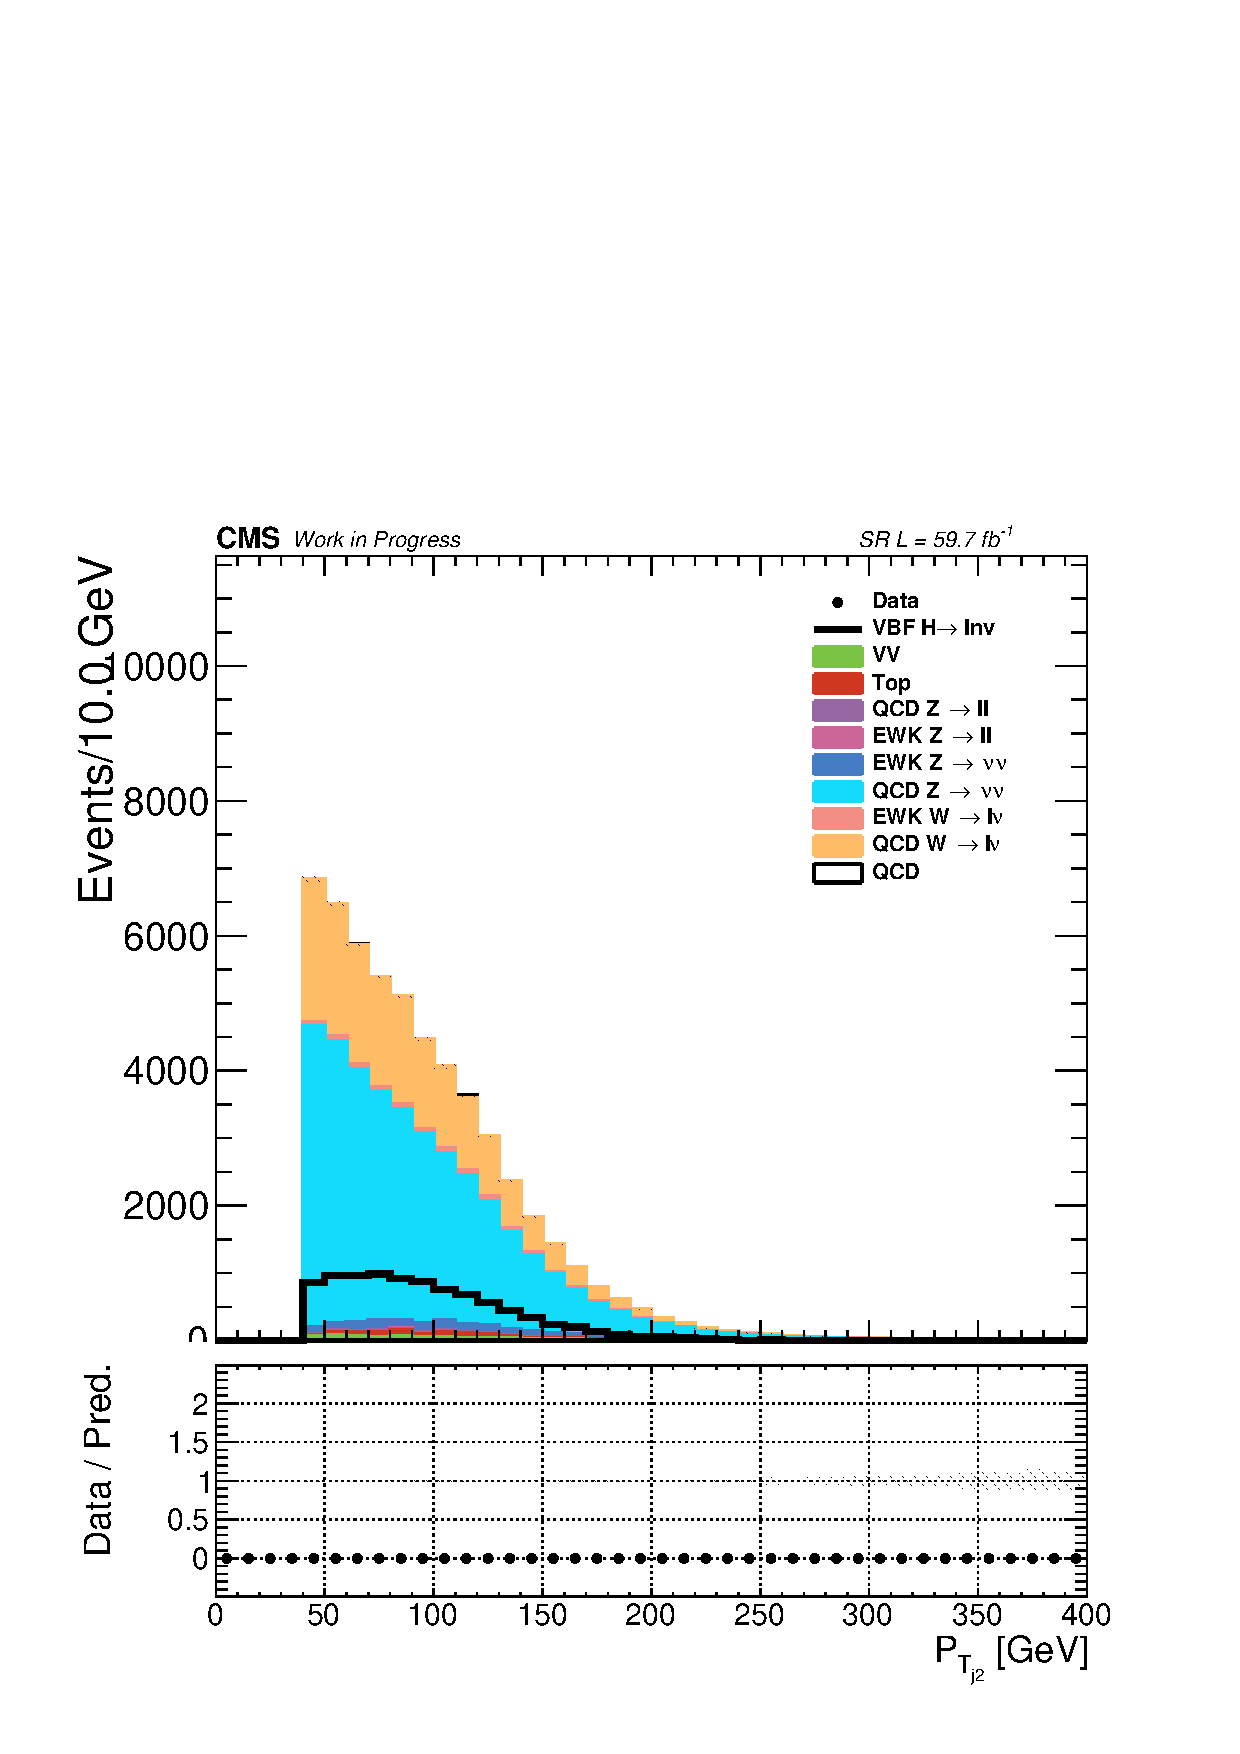
\includegraphics[width=0.49\textwidth]{Analysis_strategy/MTR_2018_SR/Subleading_jet_pt.pdf}
    }
  \caption{Distributions of $E_{T,miss}$, $M_{jj}$, $p_{T,j1}$ and $p_{T,j2}$ variables in the SR after the full MTR selection, representing the 2018 era.}
  \label{fig:2018_SR_motivation_2}
\end{figure}


\begin{figure}[htbp]
  \centering
      \subfigure[\mindphi]{
    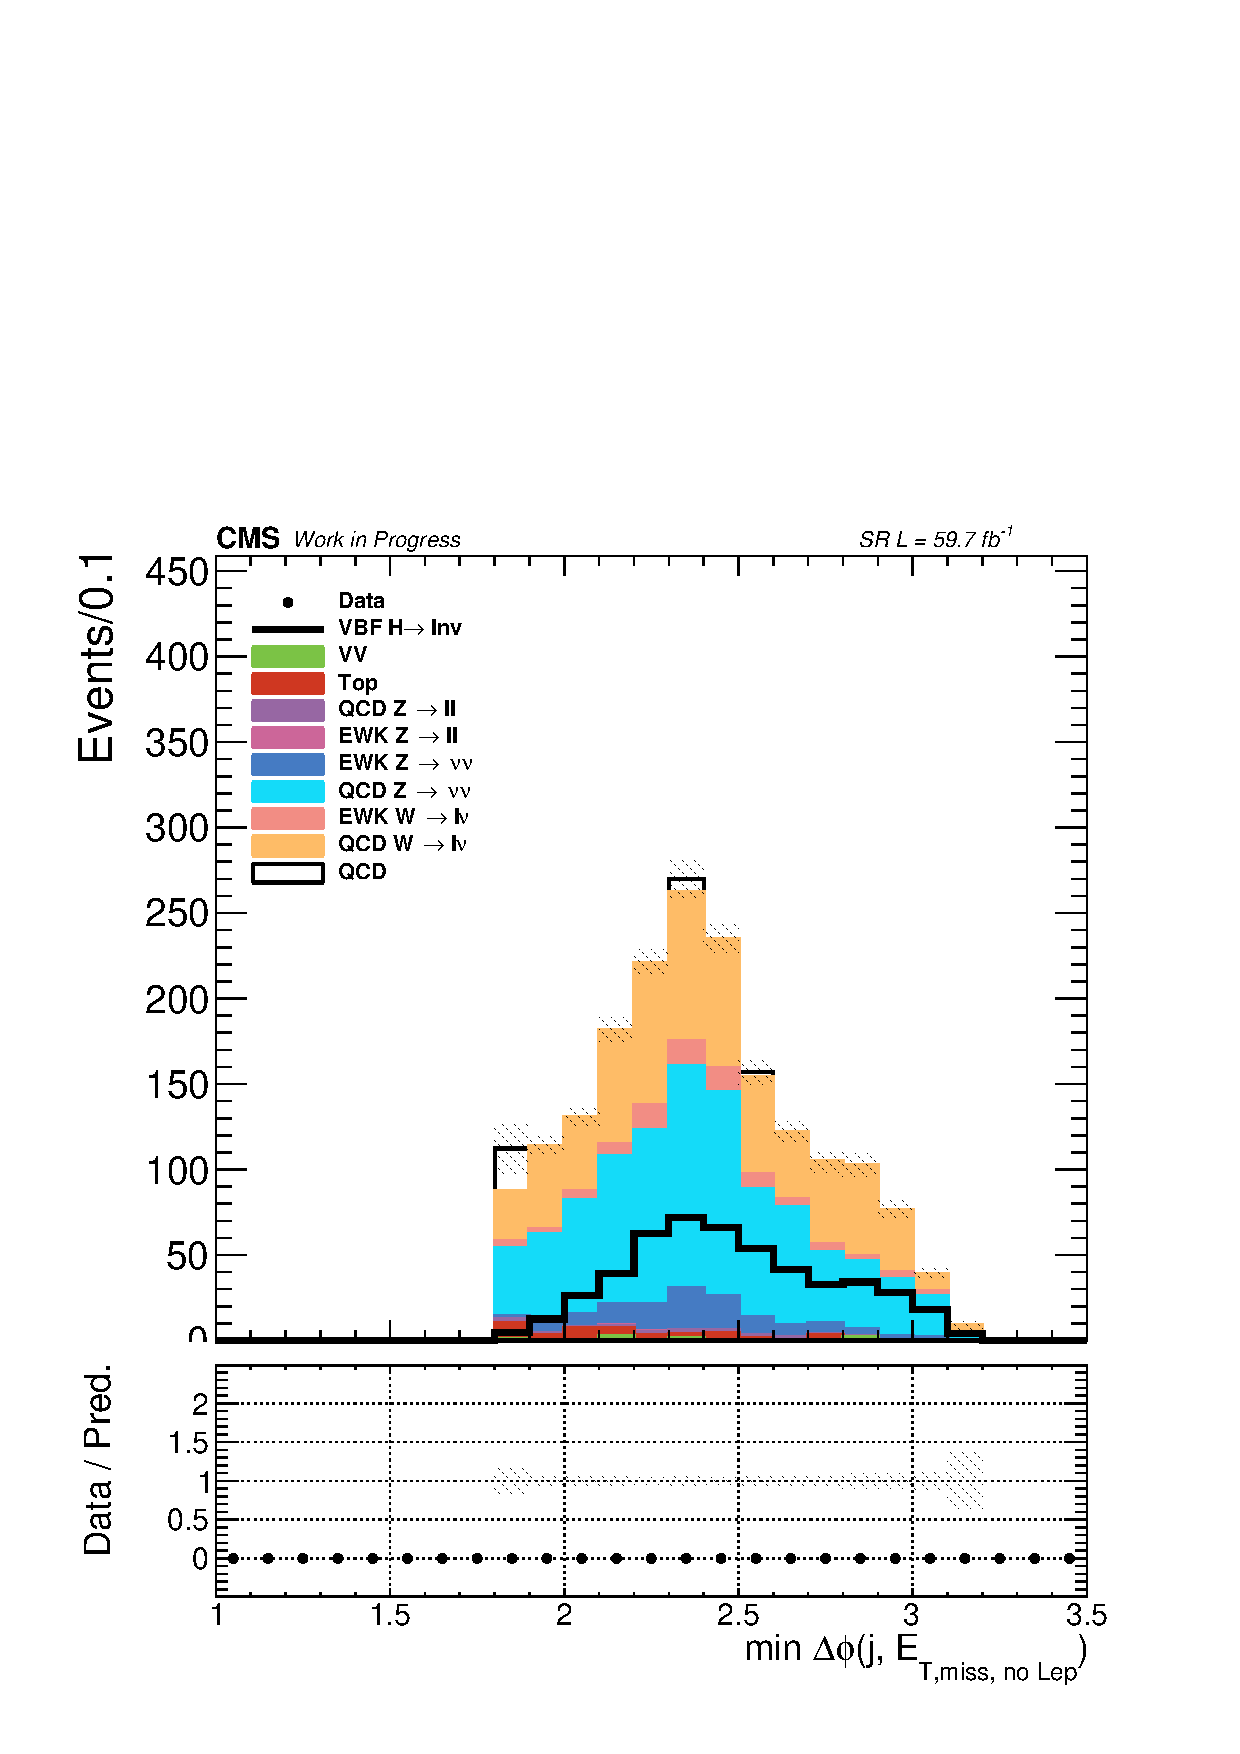
\includegraphics[width=0.49\textwidth]{Analysis_strategy/VTR_2018_SR/MetNoLep_CleanJet_mindPhi.pdf}
    }\\
    \subfigure[$\Delta\eta_{jj}$]{
    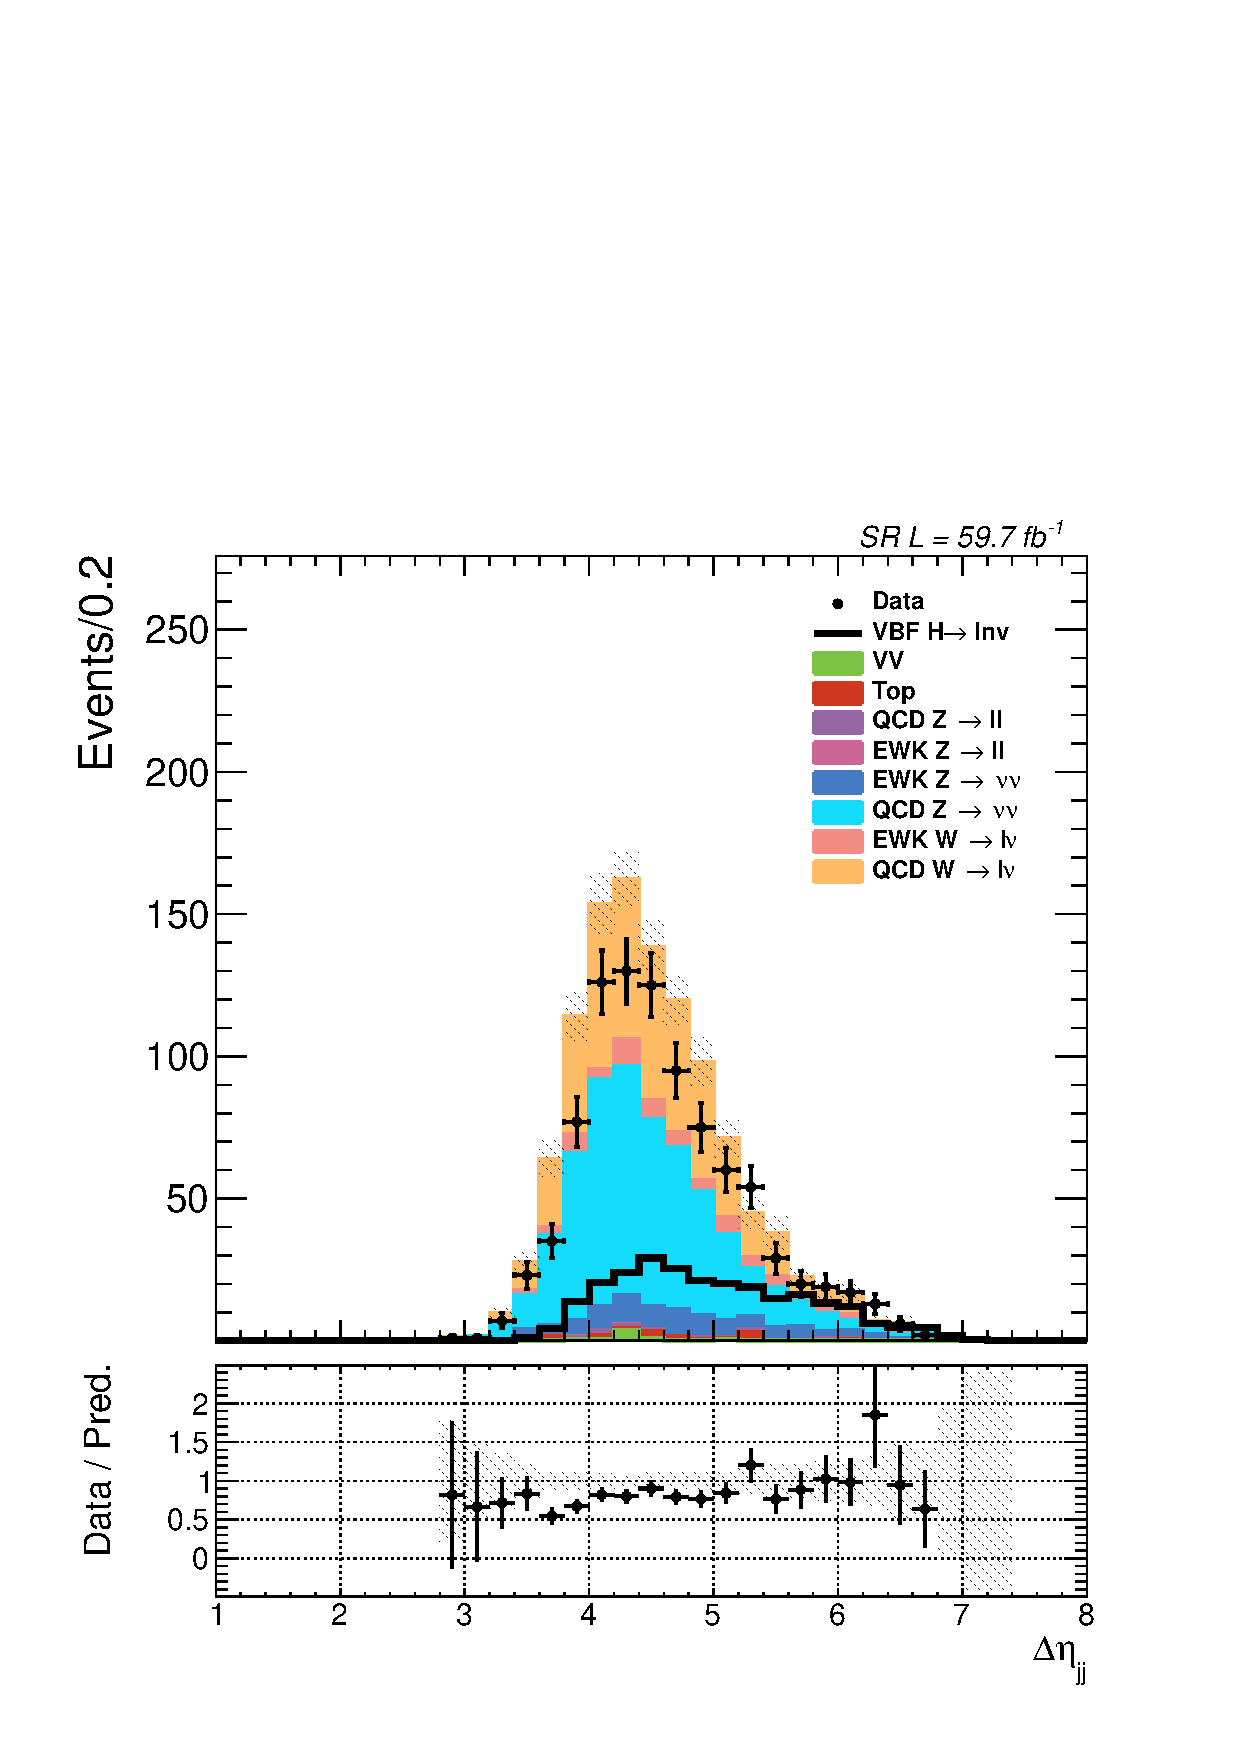
\includegraphics[width=0.49\textwidth]{Analysis_strategy/VTR_2018_SR/lMjj_leading_dEtajj.pdf}
    }
    \subfigure[$\Delta\phi_{jj}$]{
    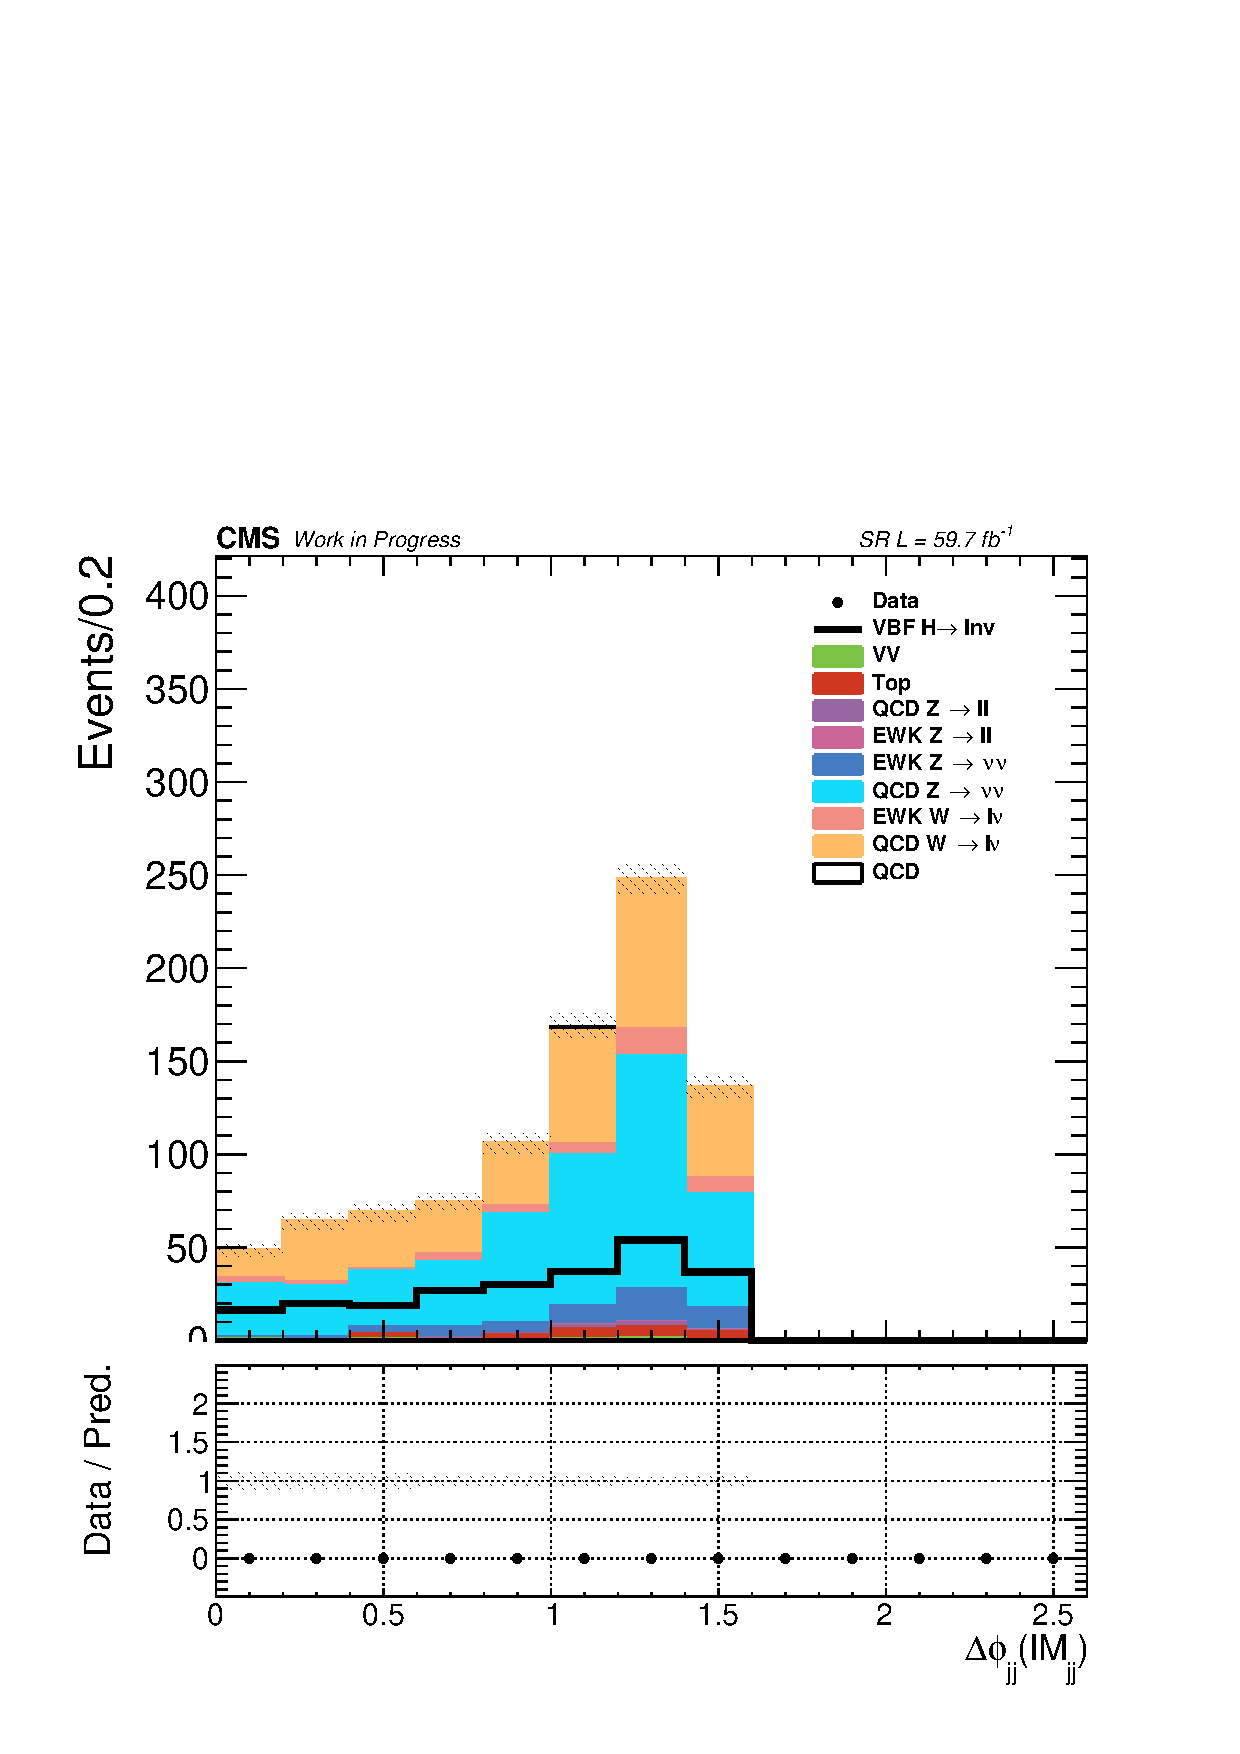
\includegraphics[width=0.49\textwidth]{Analysis_strategy/VTR_2018_SR/lMjj_leading_dPhijj.pdf}
    }
  \caption{Distributions of \mindphi, $\Delta\eta_{jj}$ and $\Delta\phi_{jj}$ variables in the SR after the full VTR selection, representing the 2018 era.}
  \label{fig:2018_VTR_SR_motivation_1}
\end{figure}
\begin{figure}[htbp]
  \centering
      \subfigure[$E_{T,miss}$]{
    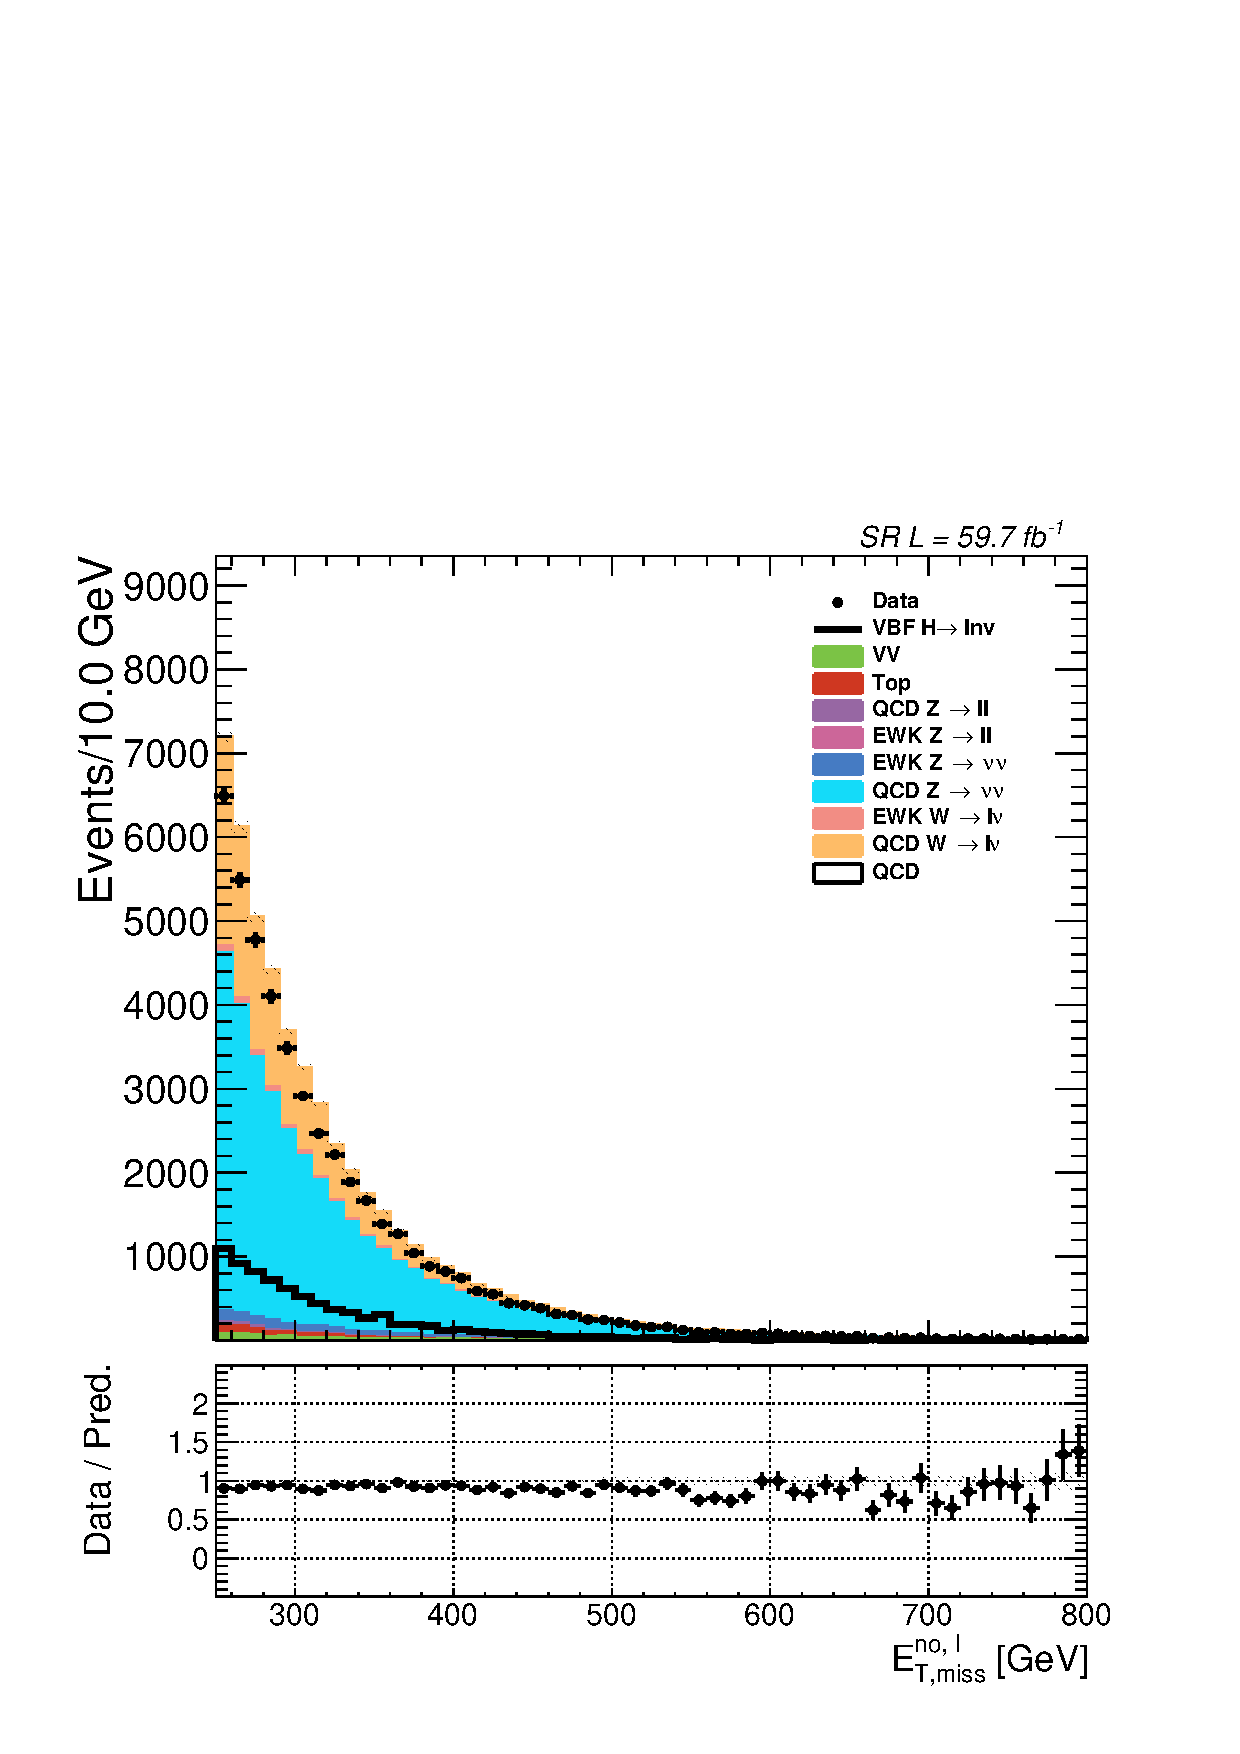
\includegraphics[width=0.49\textwidth]{Analysis_strategy/MTR_2018_SR/MetNoMu.pdf}
    }
    \subfigure[$M_{jj}$]{
    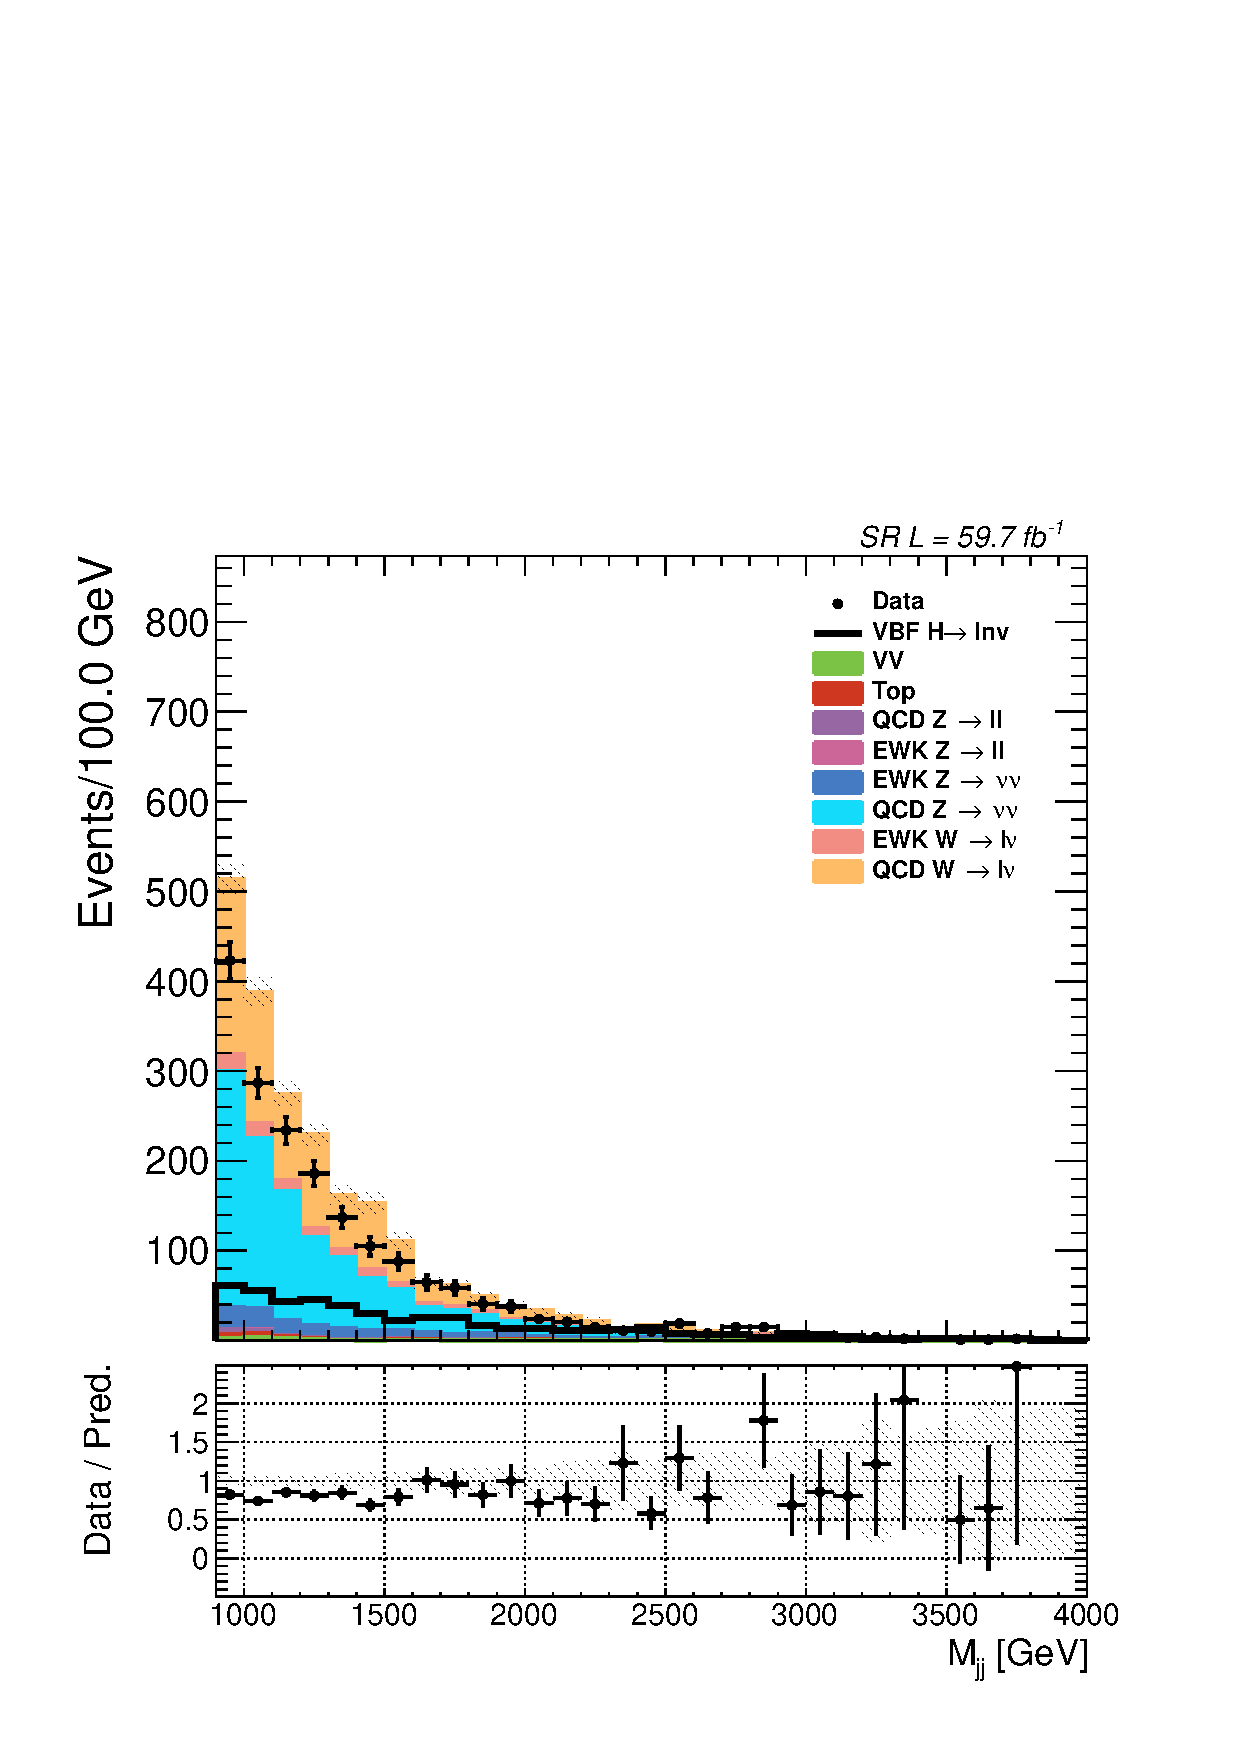
\includegraphics[width=0.49\textwidth]{Analysis_strategy/VTR_2018_SR/lMjj.pdf}
    }\\
    \subfigure[$p_{T,j1}$]{
    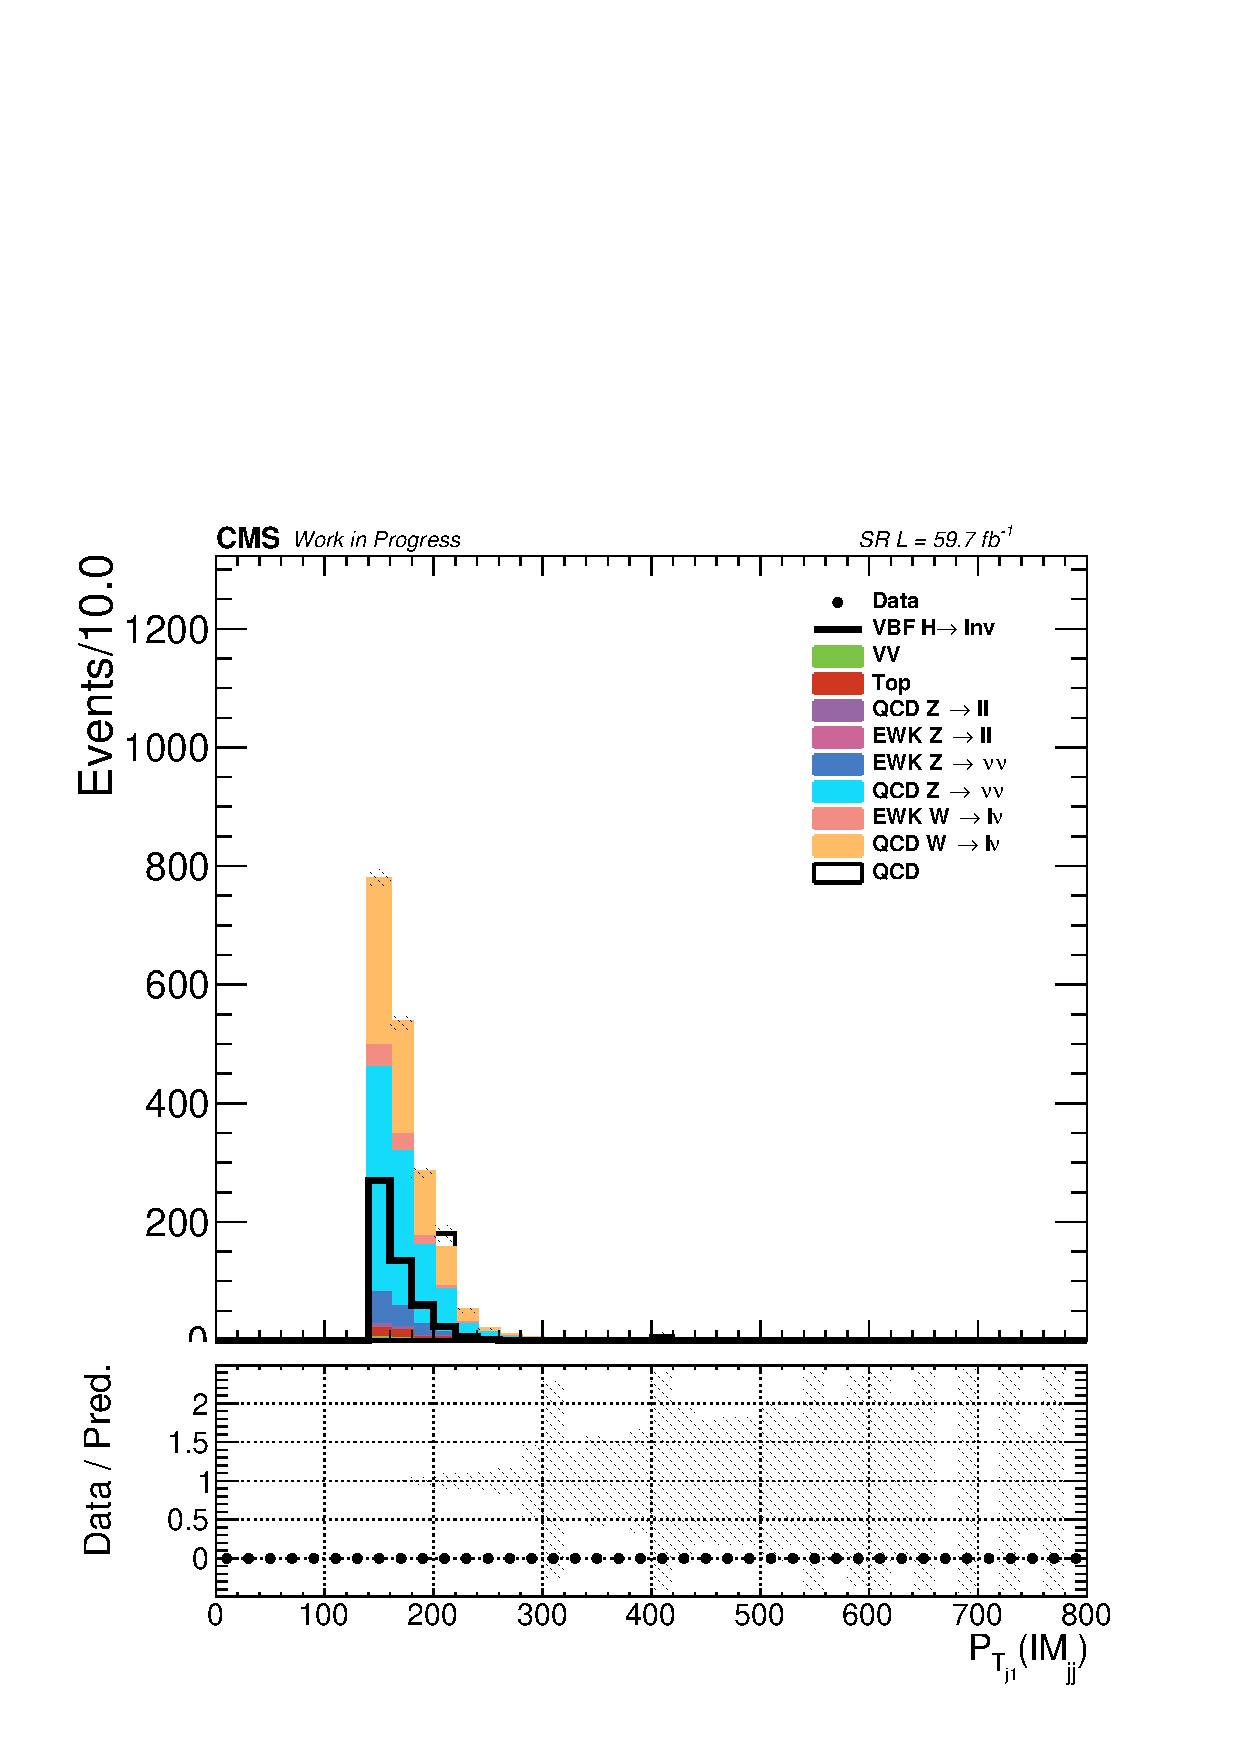
\includegraphics[width=0.49\textwidth]{Analysis_strategy/VTR_2018_SR/lMjj_Leading_jet_pt.pdf}
    }
    \subfigure[$p_{T,j2}$]{
    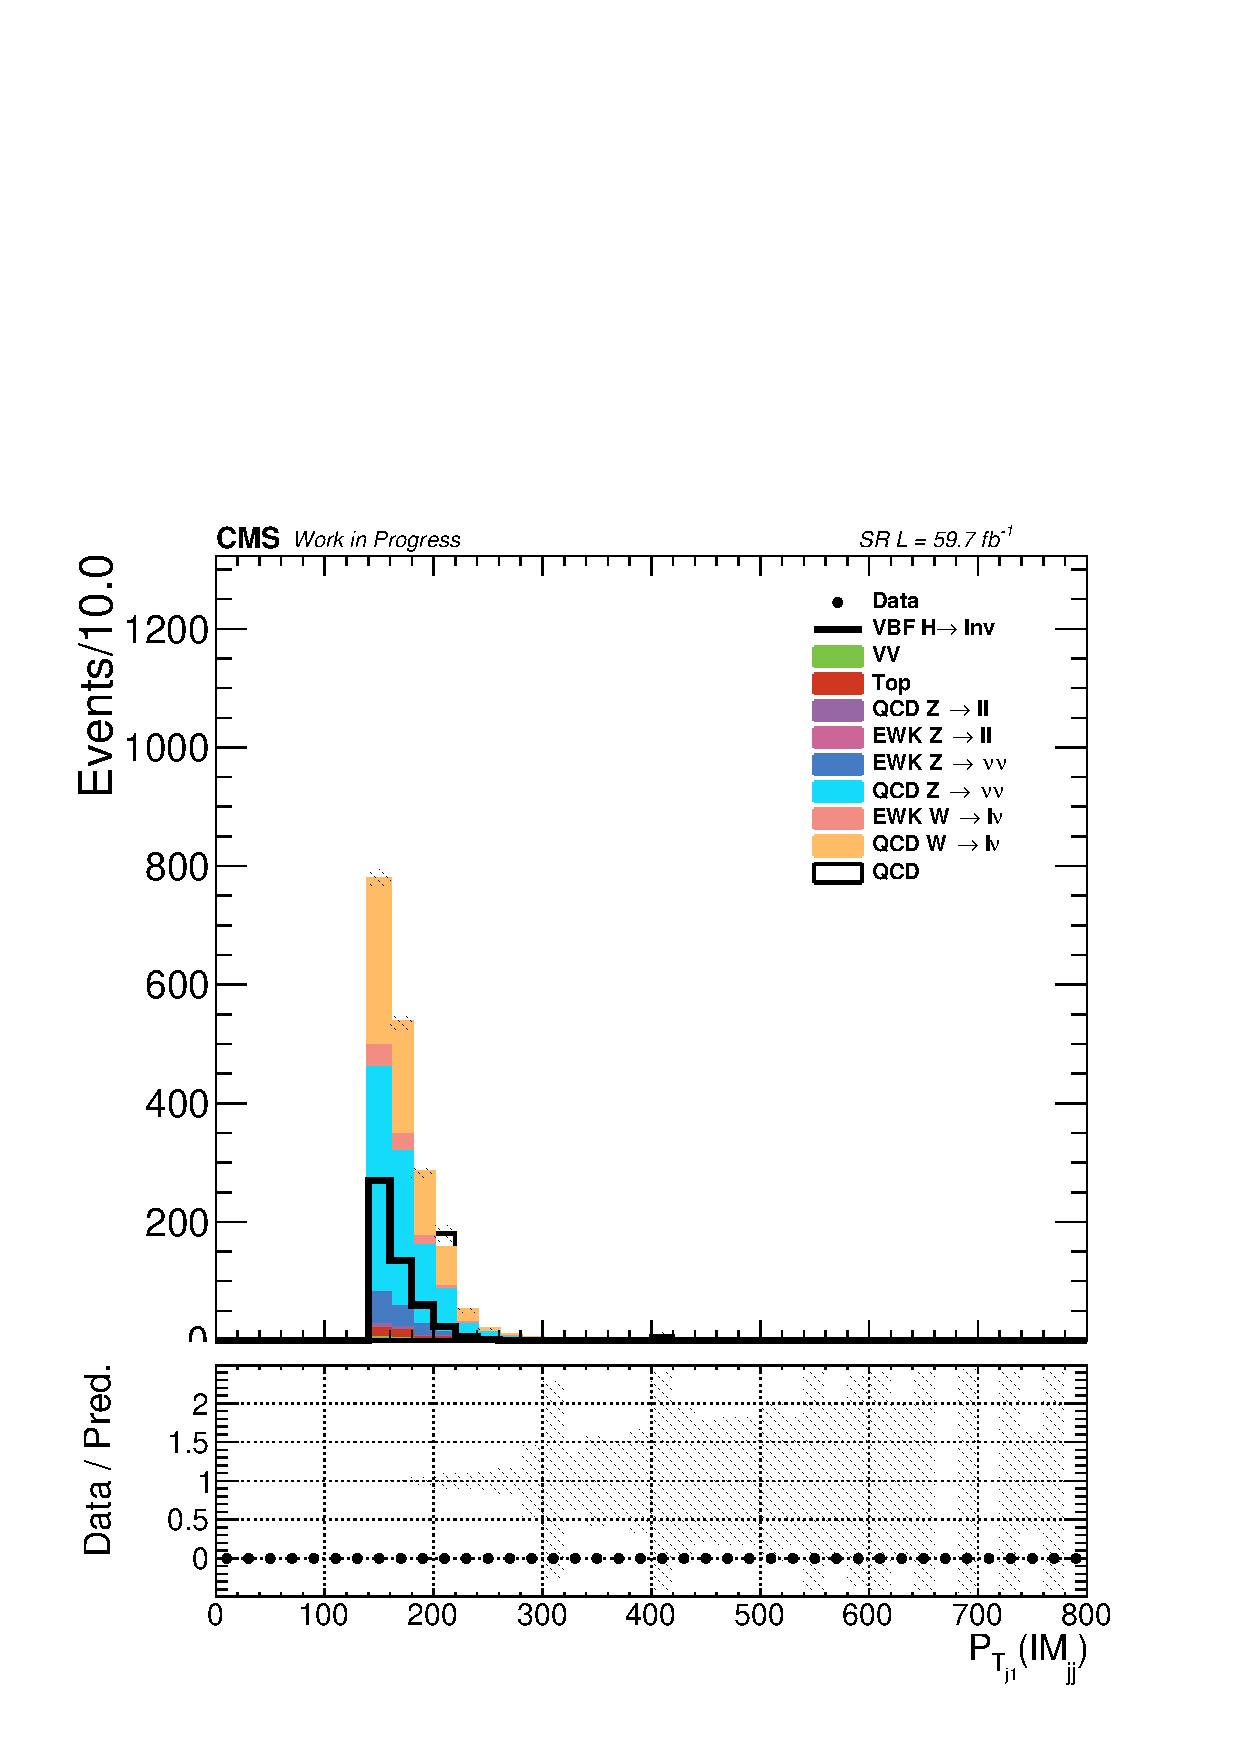
\includegraphics[width=0.49\textwidth]{Analysis_strategy/VTR_2018_SR/lMjj_Leading_jet_pt.pdf}
    }
  \caption{Distributions of $E_{T,miss}$, $M_{jj}$, $p_{T,j1}$ and $p_{T,j2}$ variables in the SR after the full VTR selection, representing the 2018 era.}
  \label{fig:2018_VTR_SR_motivation_2}
\end{figure}


\begin{figure}[htbp]
  \centering
    \subfigure[$p_{T,j_1}$ - MTR]{
    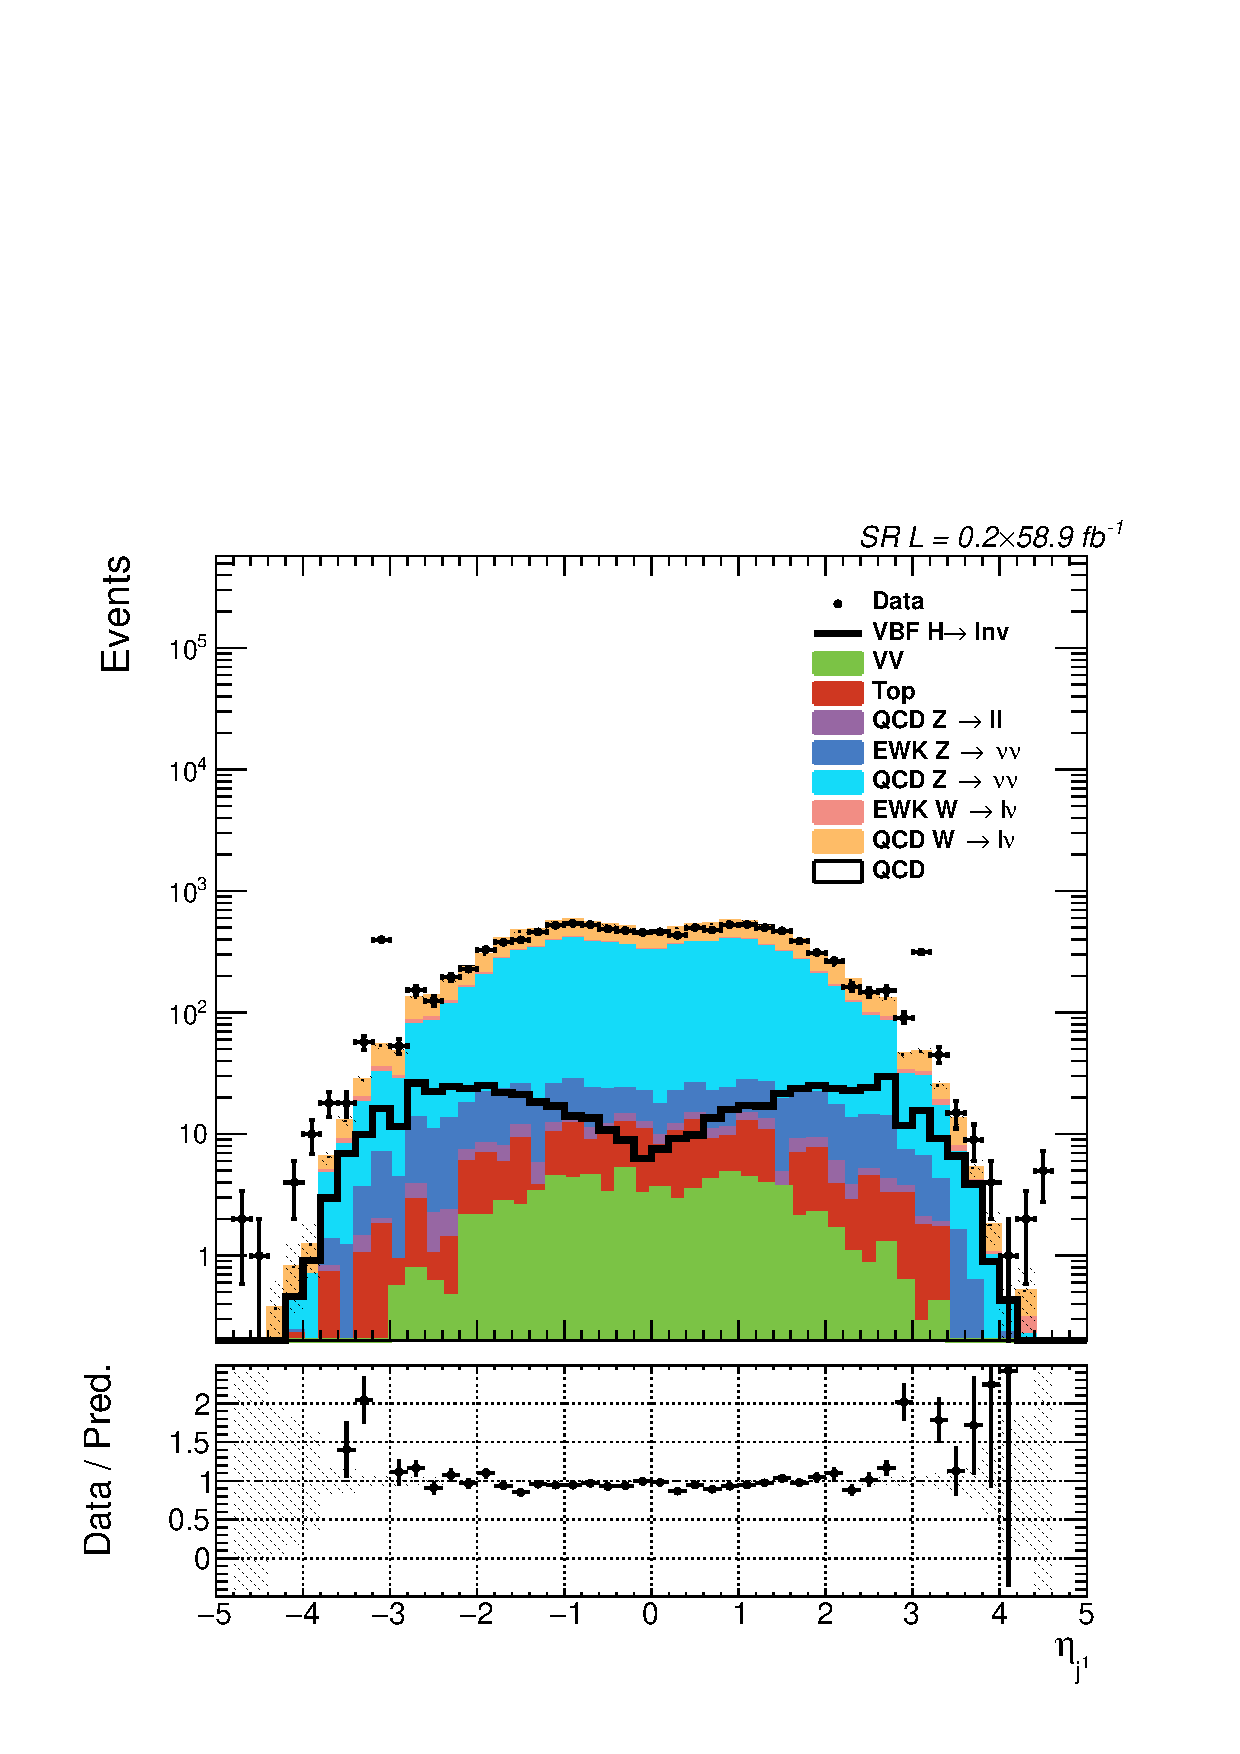
\includegraphics[width=0.49\textwidth]{Analysis_strategy/2018_preHornCut/Leading_jet_eta_log.pdf}
    }
    \subfigure[$p_{T,j_2}$ - MTR]{
    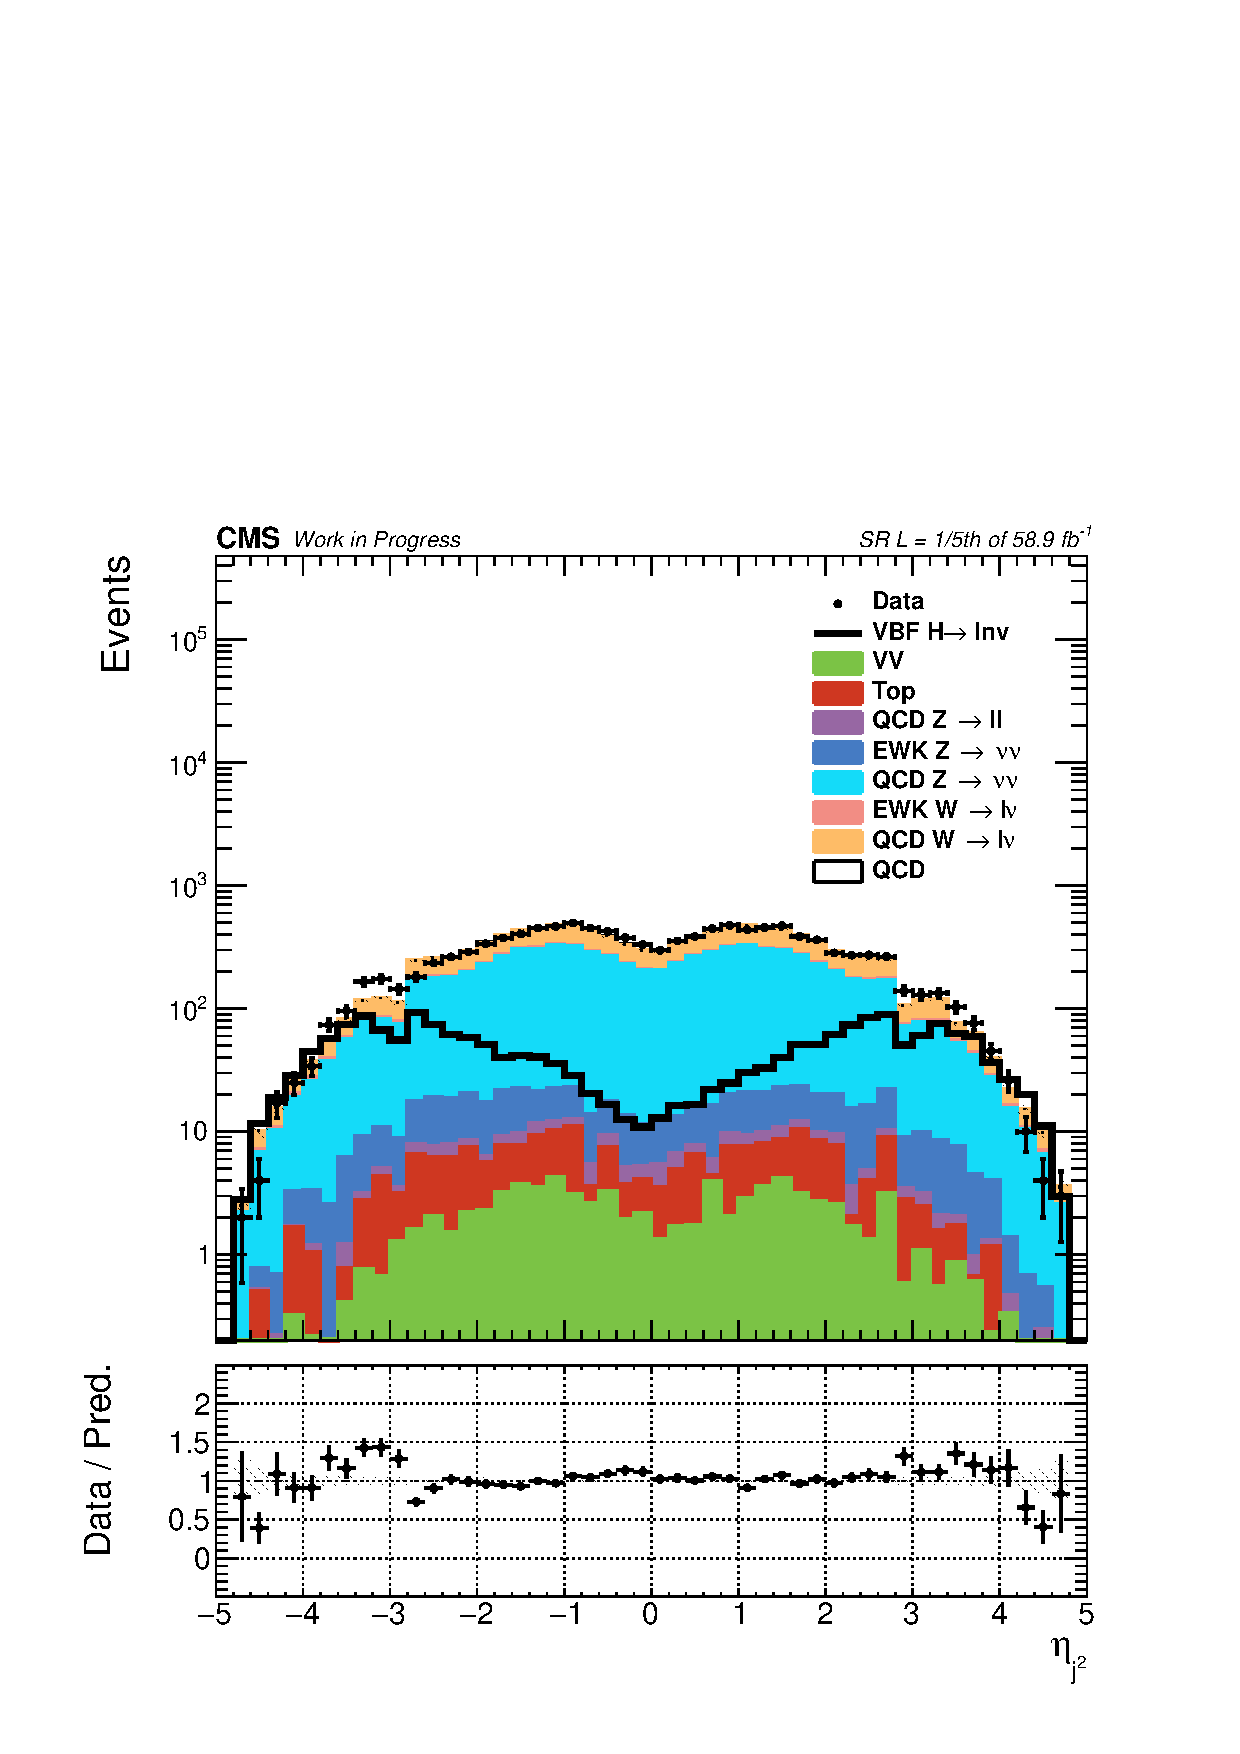
\includegraphics[width=0.49\textwidth]{Analysis_strategy/2018_preHornCut/Subleading_jet_eta_log.pdf}
    }\\
    \subfigure[$p_{T,j_1}$ - VTR]{
    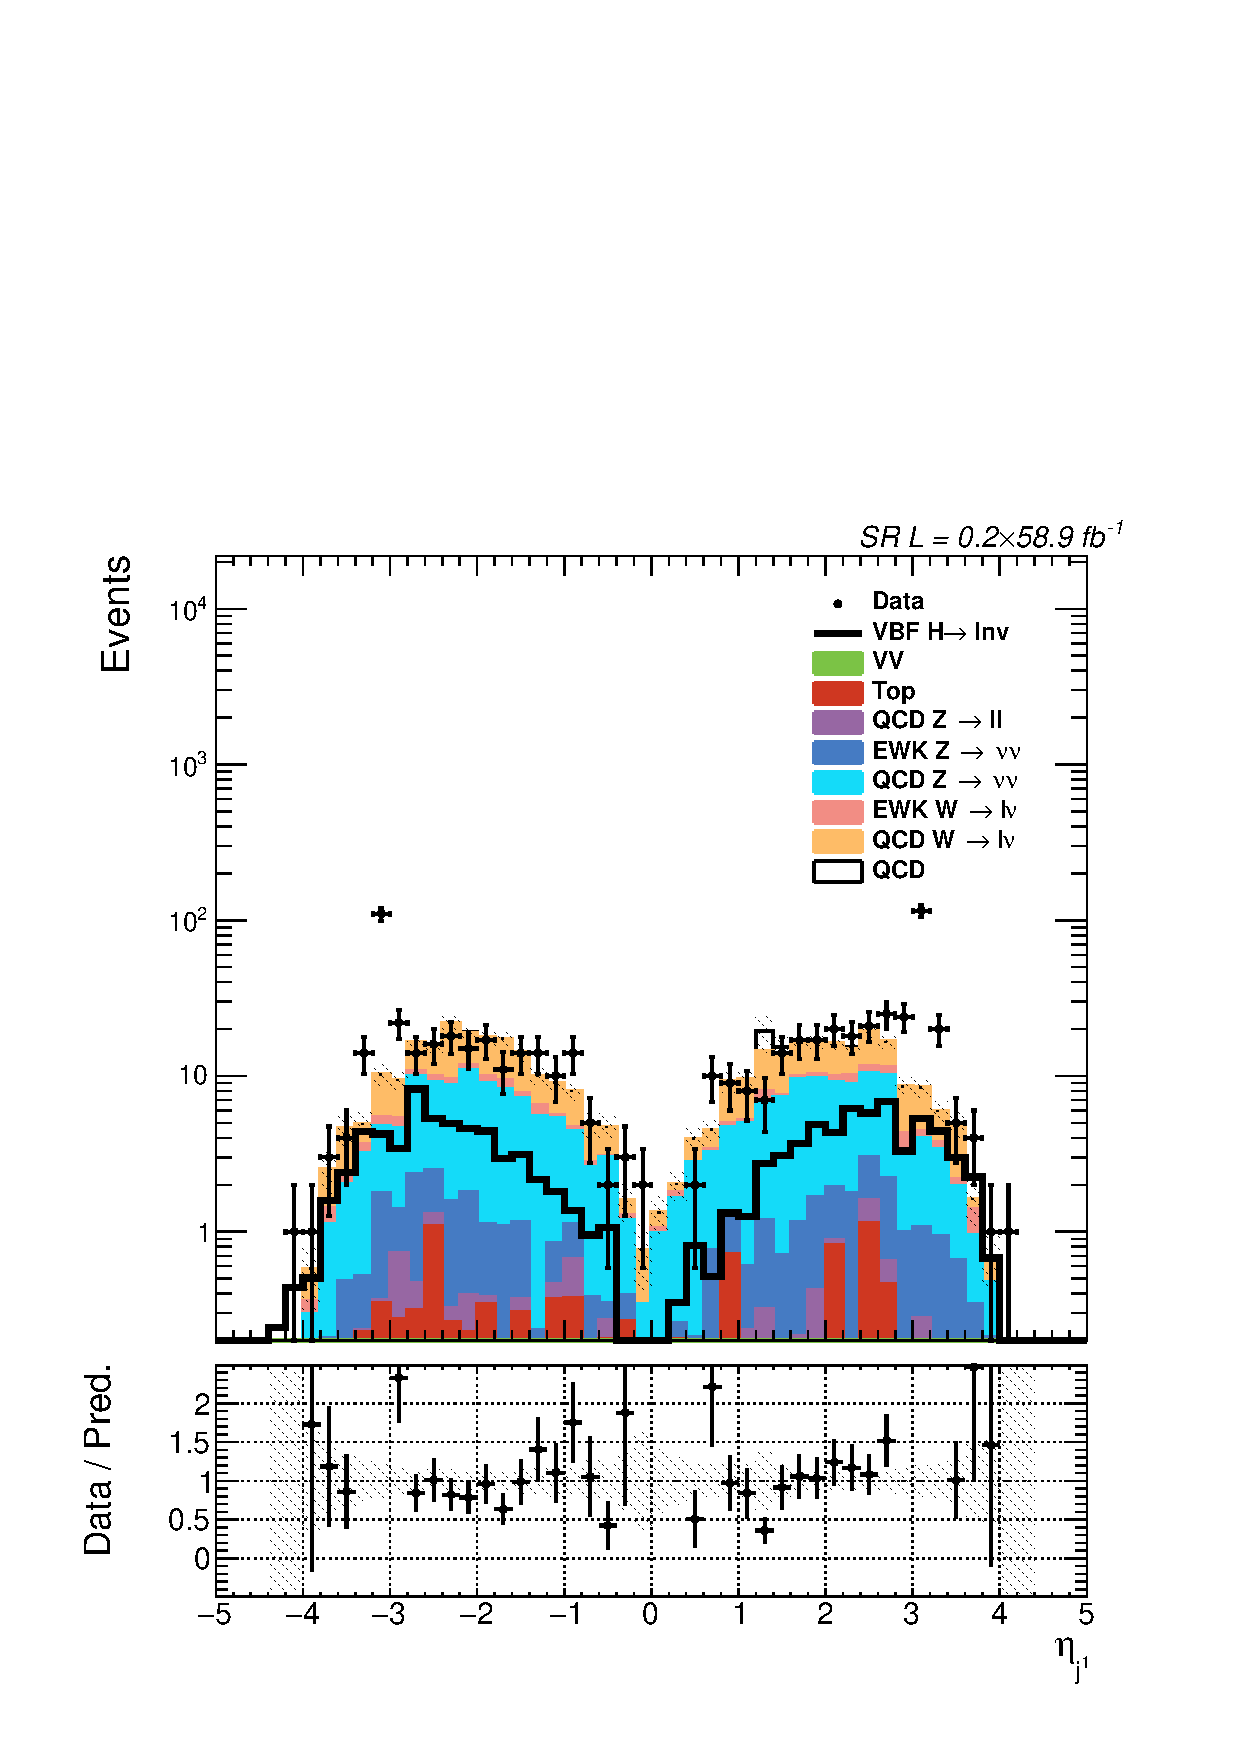
\includegraphics[width=0.49\textwidth]{Analysis_strategy/2018_preHornCut/VTRLeading_jet_eta_log.pdf}
    }
    \subfigure[$p_{T,j_2}$ - VTR]{
    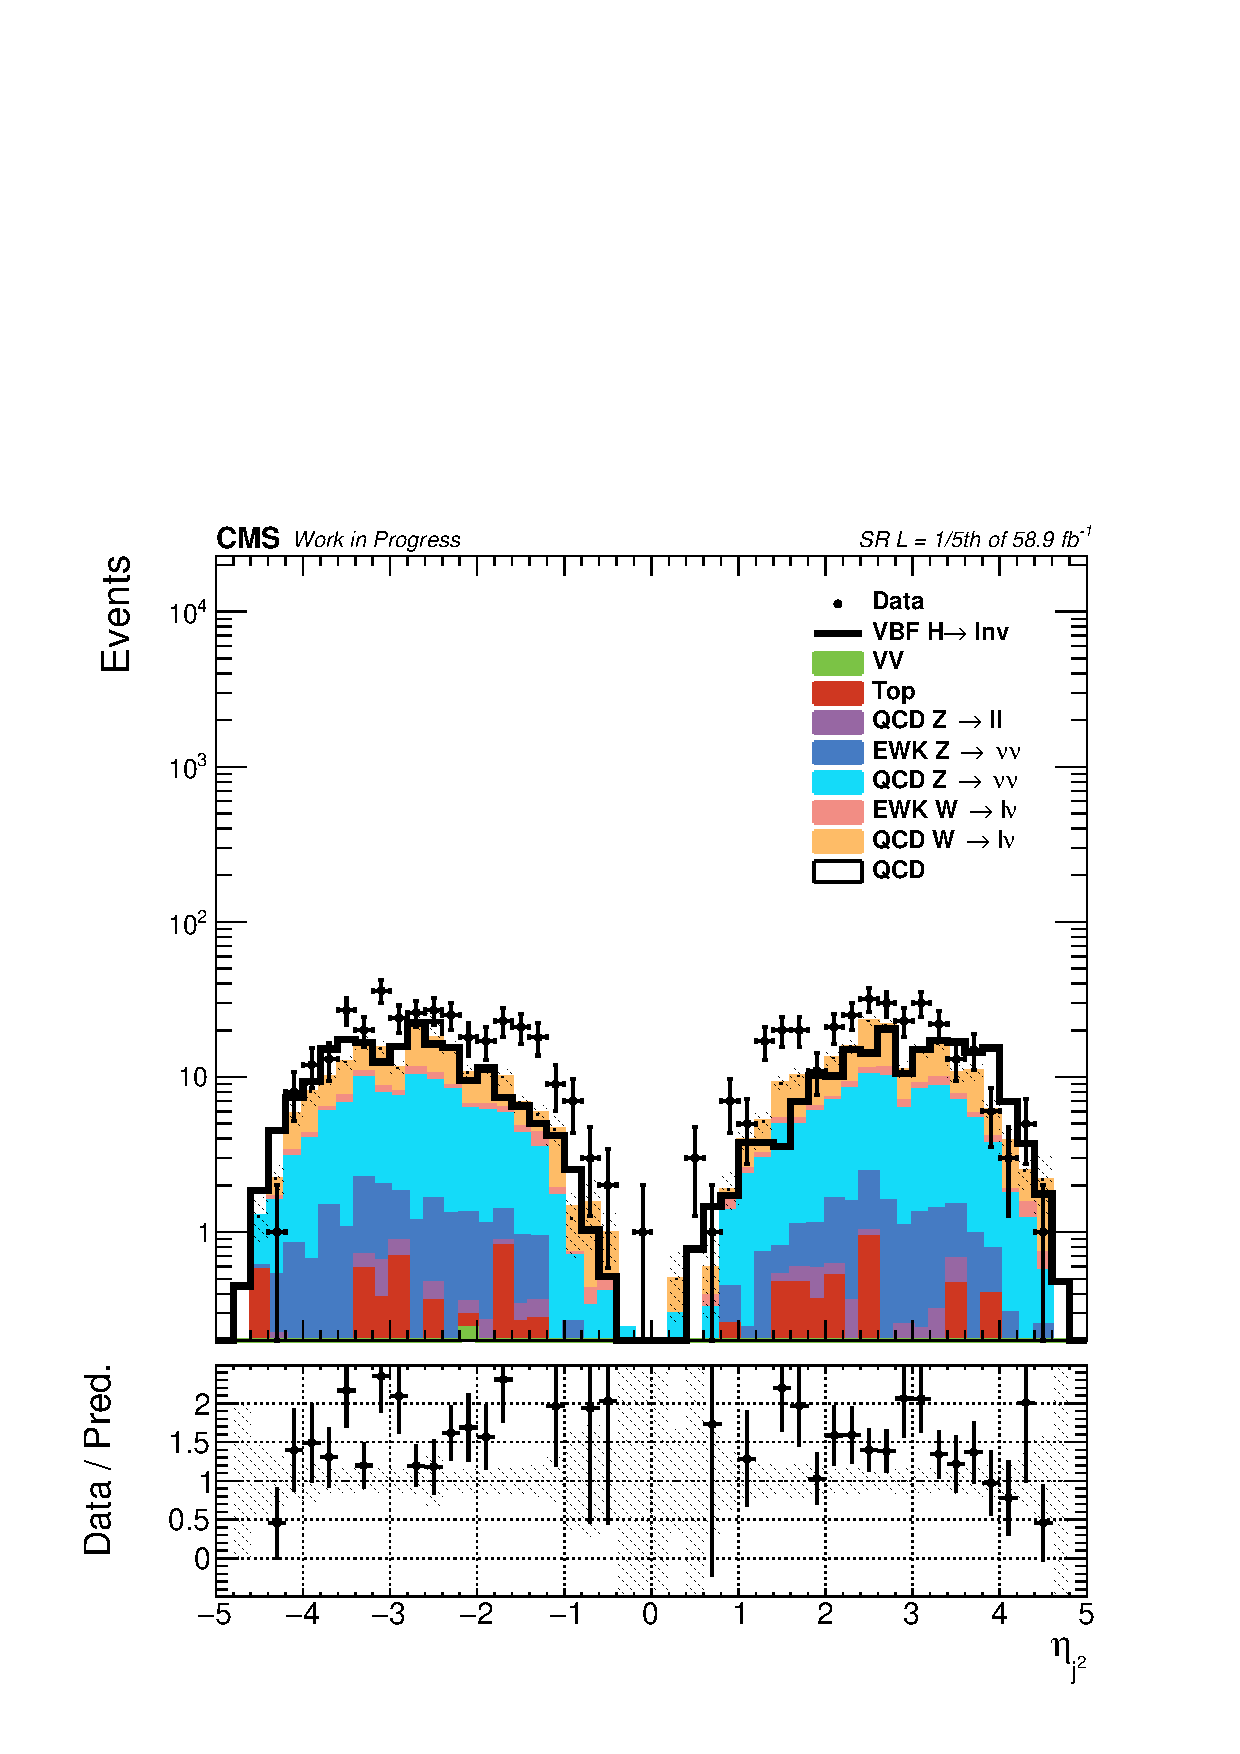
\includegraphics[width=0.49\textwidth]{Analysis_strategy/2018_preHornCut/VTRSubleading_jet_eta_log.pdf}
    }
  \caption{Distributions of $p_{T,j1}$ (left) and $p_{T,j2}$ (right) variables in the signal region after the unbinding of 1/5th of the 2018 data. Both MTR (top) and VTR (bottom) categories are presented.}
  \label{fig:jet_eta_preHornCut_2018}
\end{figure}




\begin{figure}[htbp]
  \centering
    \subfigure[$p_{T,j_1}$ - MTR]{
    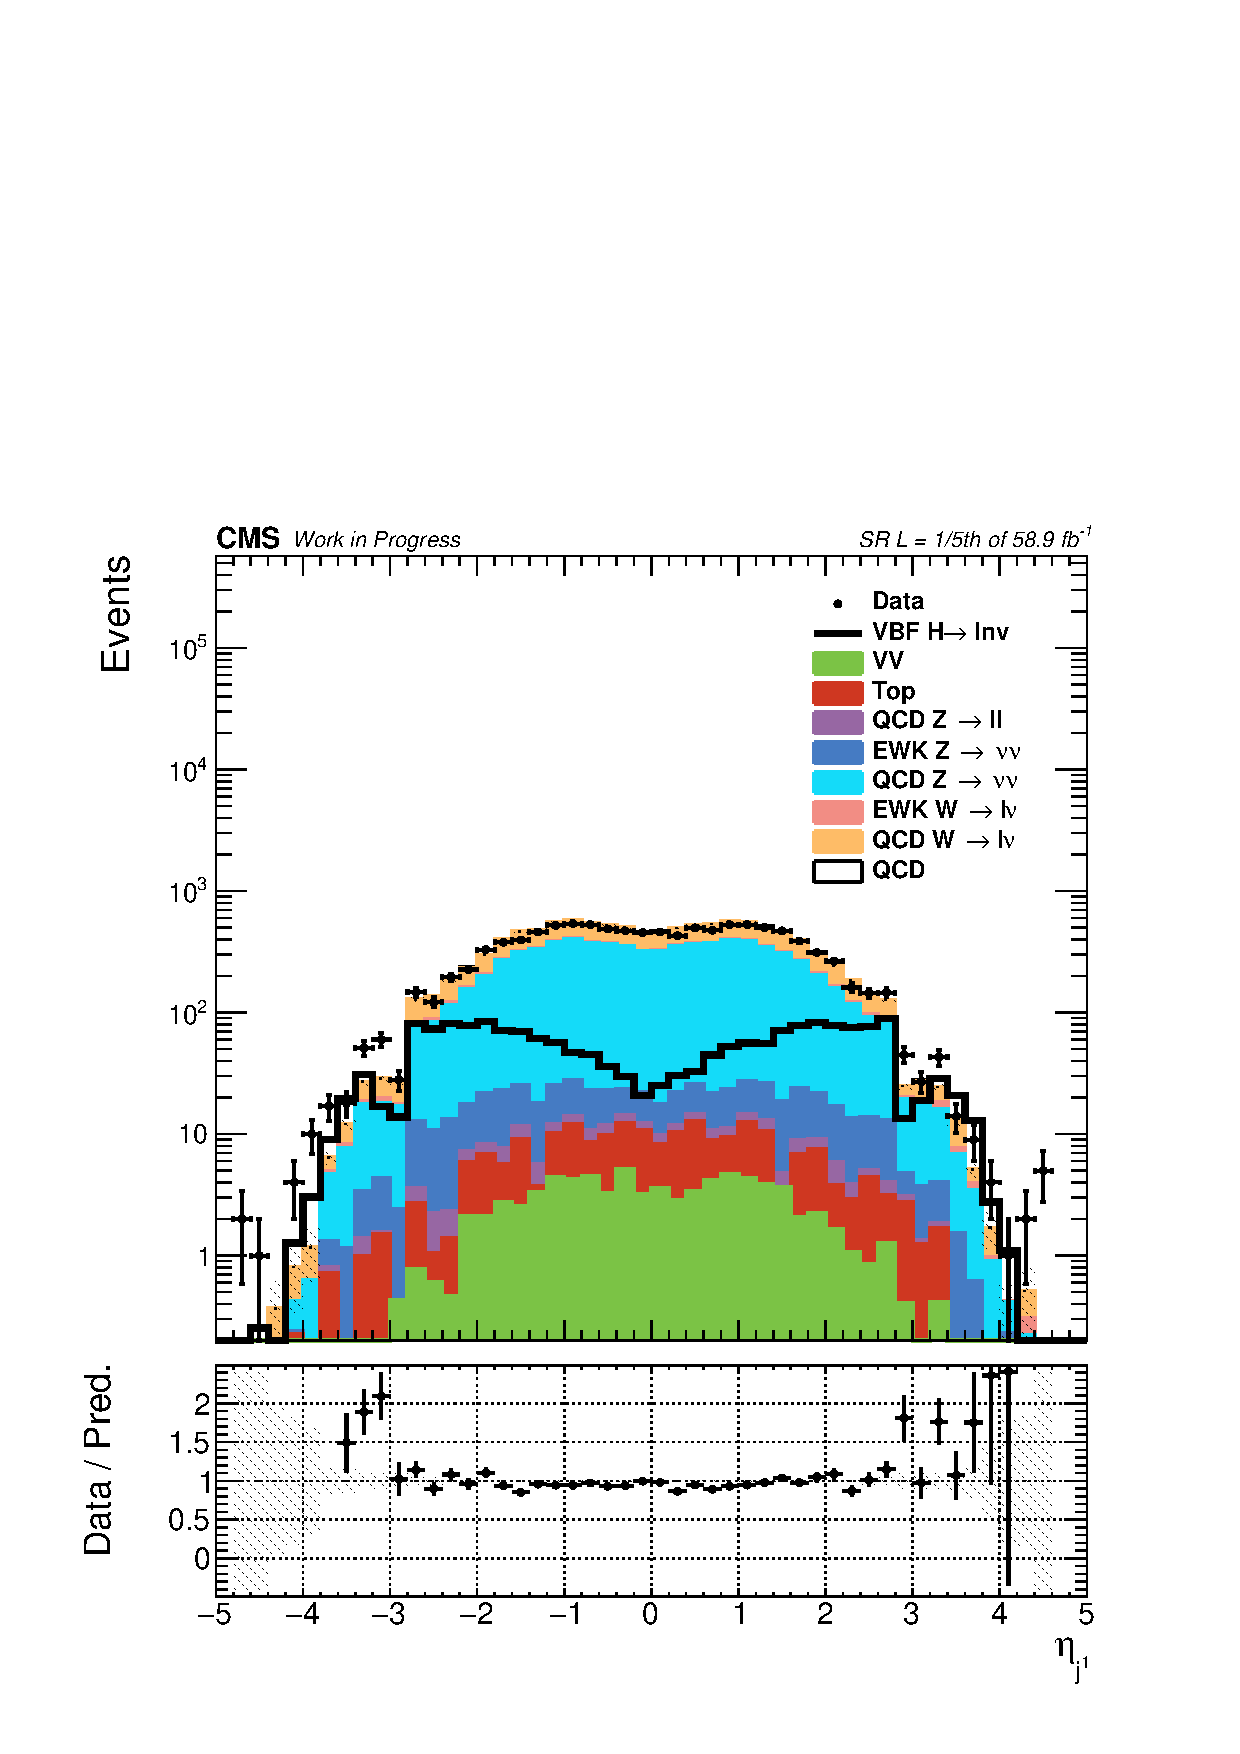
\includegraphics[width=0.49\textwidth]{Analysis_strategy/2018_postHornCut/Leading_jet_eta_log.pdf}
    }
    \subfigure[$p_{T,j_2}$ - MTR]{
    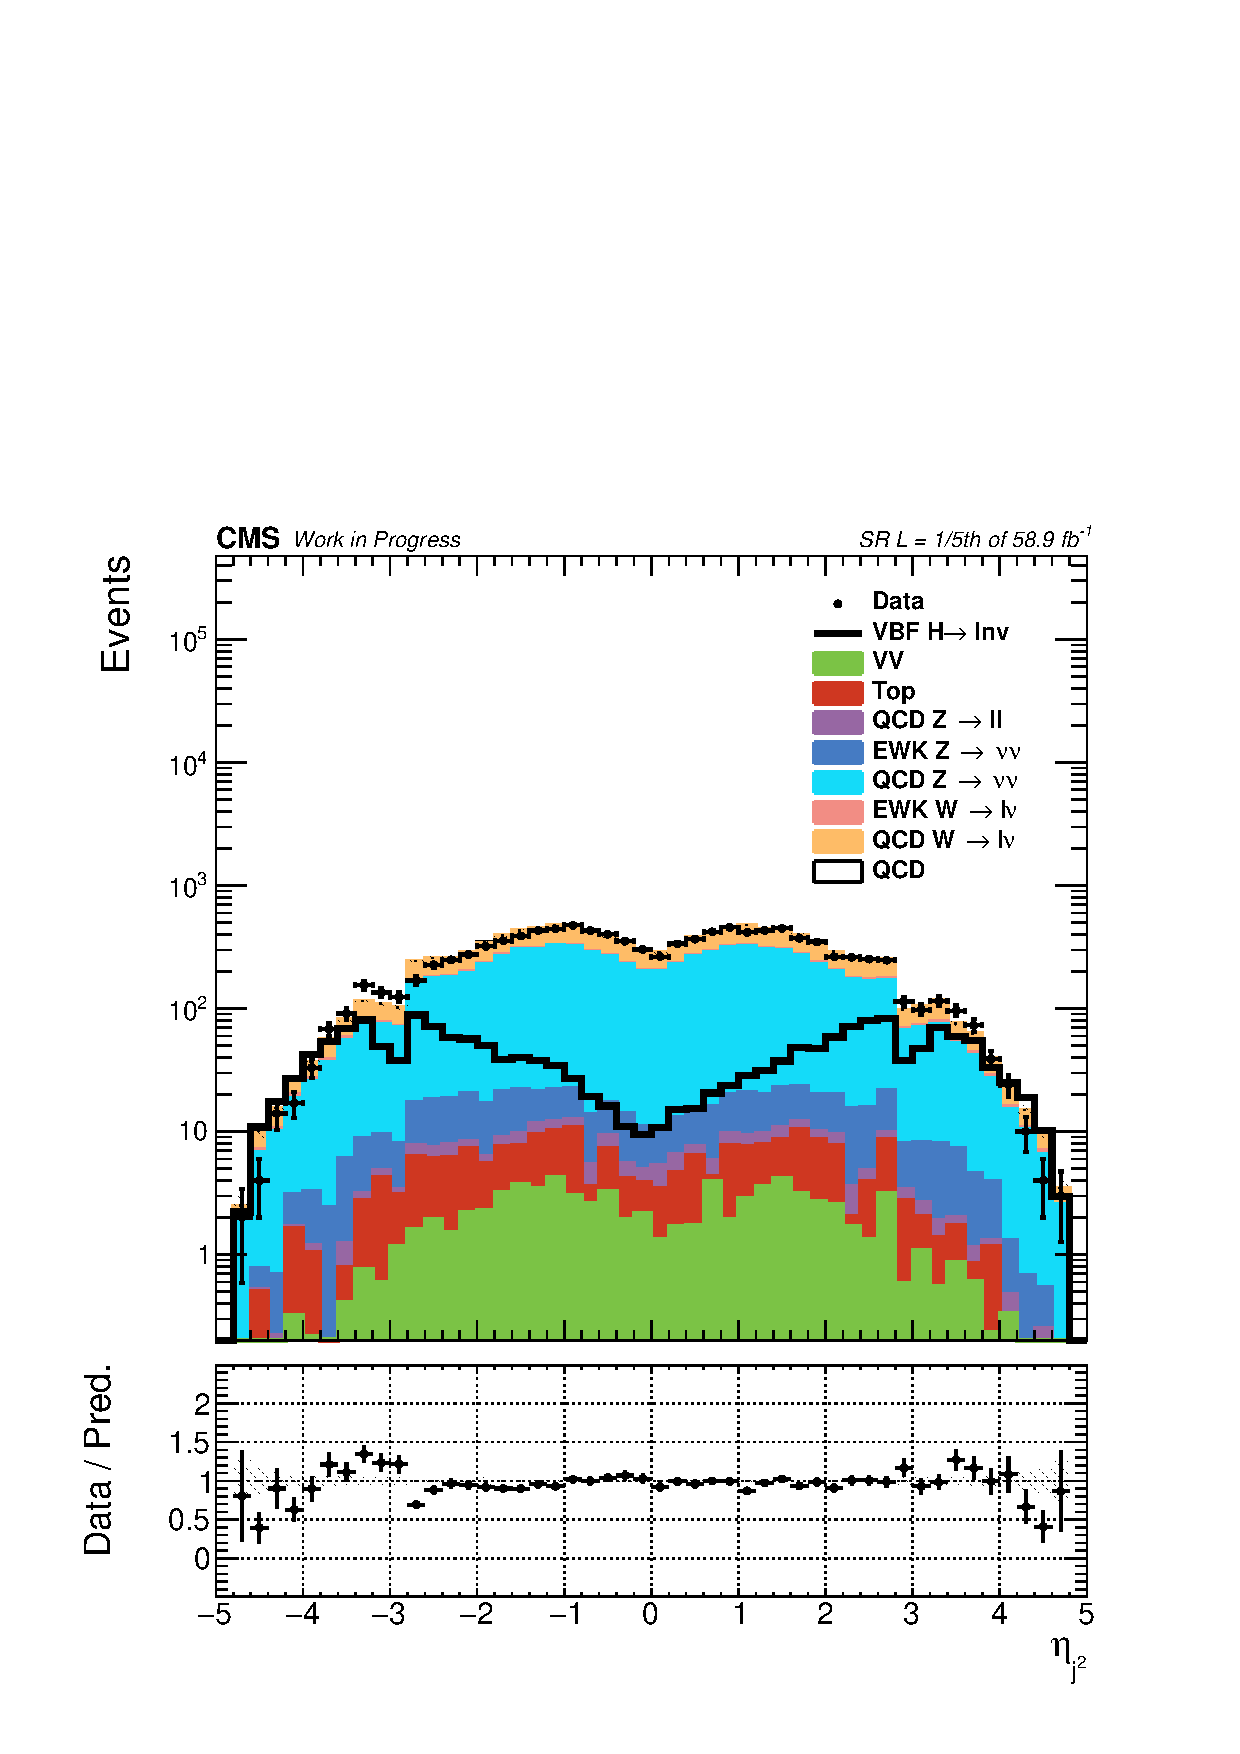
\includegraphics[width=0.49\textwidth]{Analysis_strategy/2018_postHornCut/Subleading_jet_eta_log.pdf}
    }\\
    \subfigure[$p_{T,j_1}$ - VTR]{
    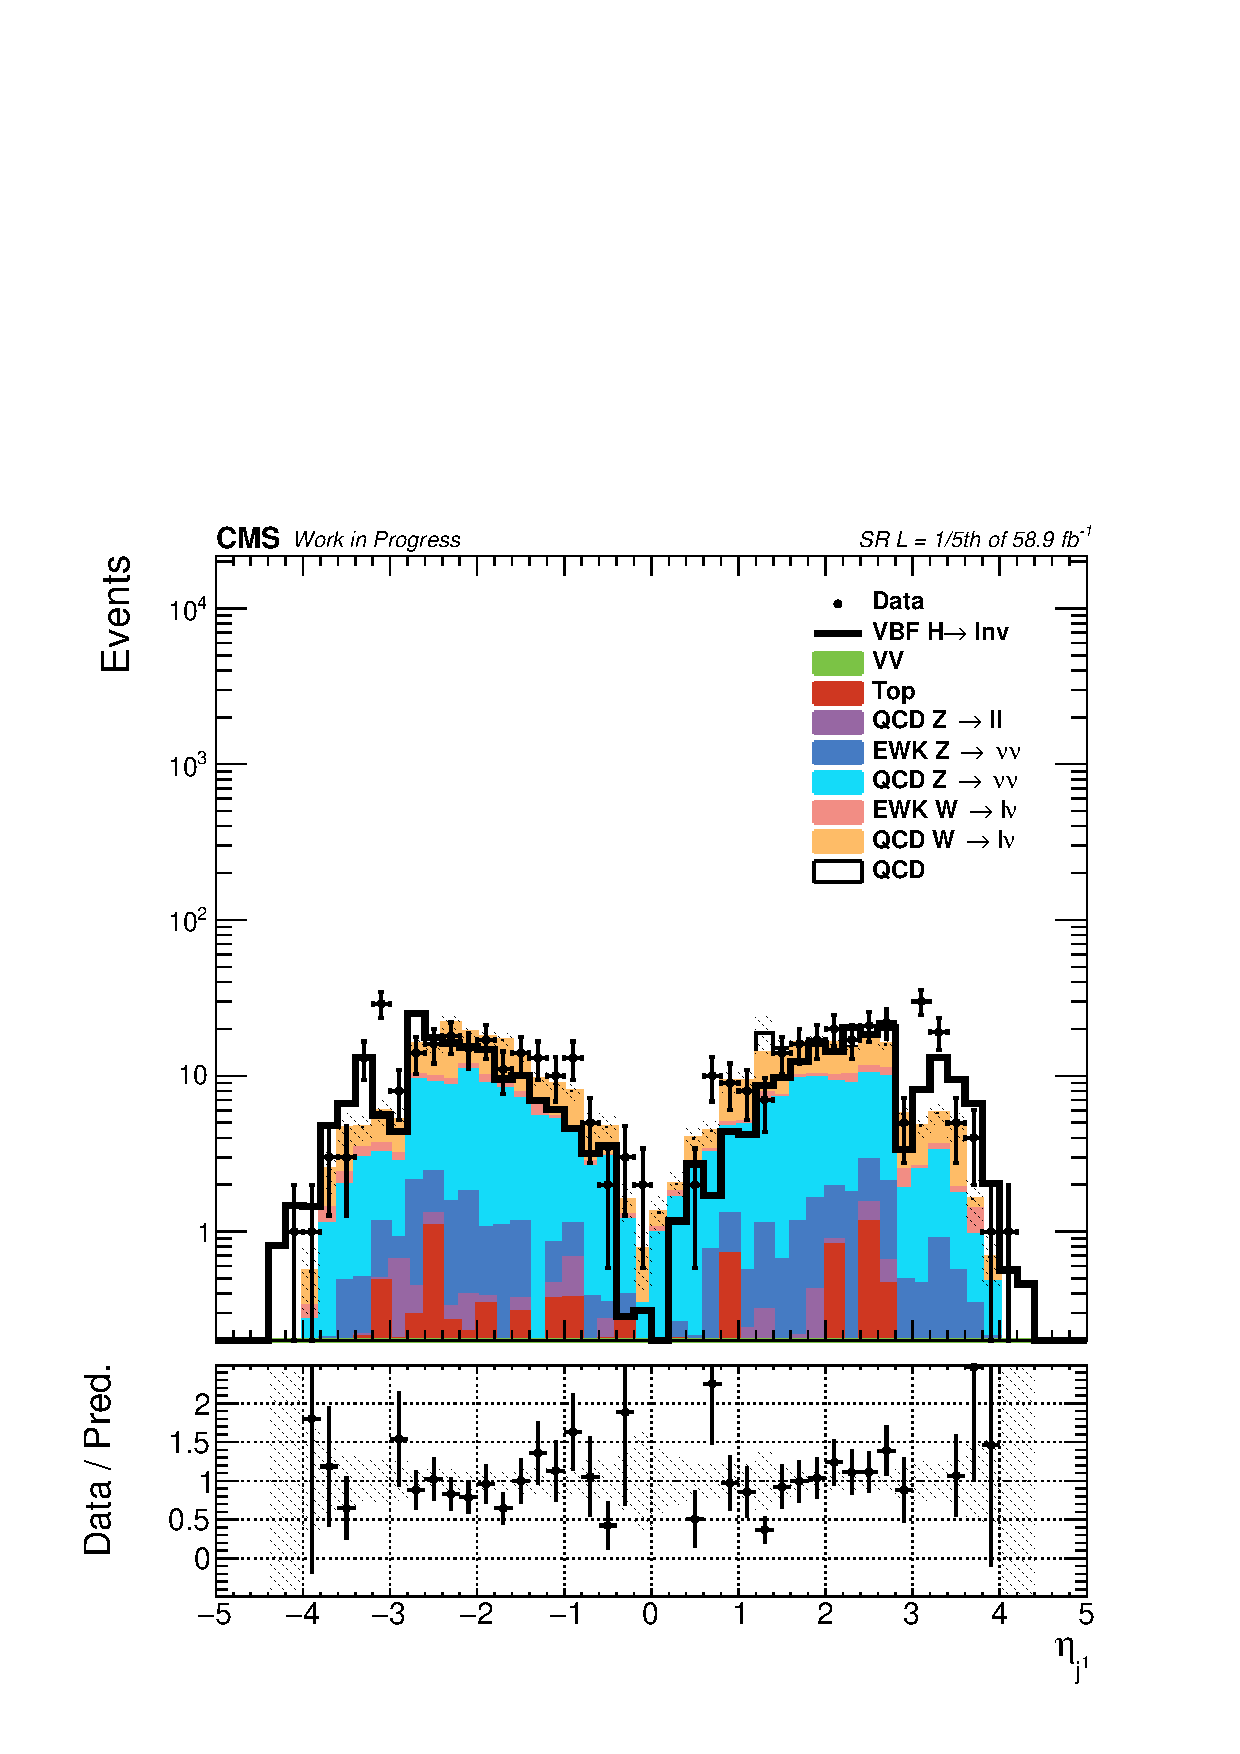
\includegraphics[width=0.49\textwidth]{Analysis_strategy/2018_postHornCut/VTRLeading_jet_eta_log.pdf}
    }
    \subfigure[$p_{T,j_2}$ - VTR]{
    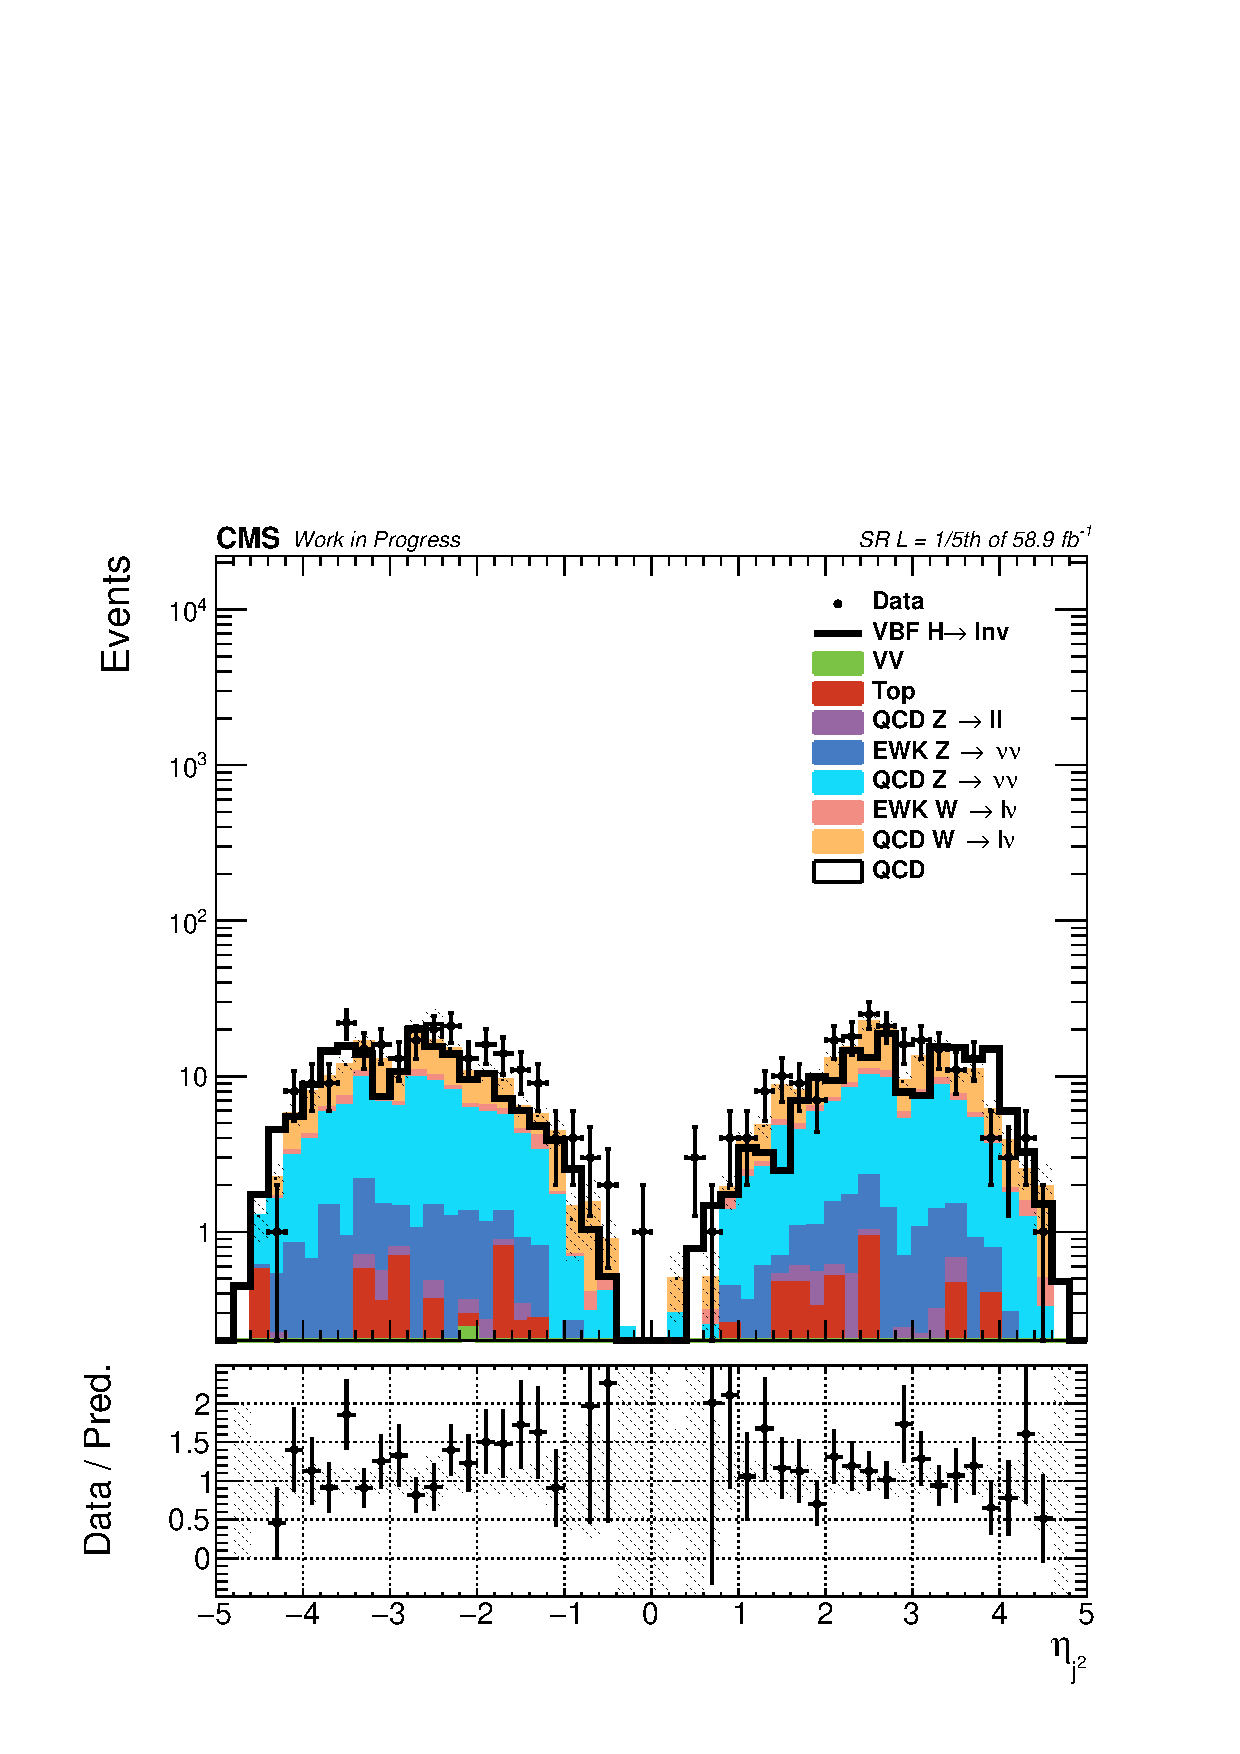
\includegraphics[width=0.49\textwidth]{Analysis_strategy/2018_postHornCut/VTRSubleading_jet_eta_log.pdf}
    }
  \caption{Distributions of $p_{T,j1}$ (left) and $p_{T,j2}$ (right) variables in the signal region after the unbinding of 1/5th of the 2018 data and the mitigation of the jet "horns" effect. Both MTR (top) and VTR (bottom) categories are presented.}
  \label{fig:jet_eta_postHornCut_2018}
\end{figure}




\section{Additional information on dedicated CRs}
\label{app:CRs}
\hspace{10pt} Supplementing the discussion presented in Section~\ref{sec:double_muon}, Figure~\ref{fig:Zmumu_noHEM} shows the absence of any effect coming from the HEM problem for the double lepton region (MTR category used as the example).

\begin{figure}[htbp]
  \centering
    \subfigure[$E_{T,miss}$ - MTR]{
    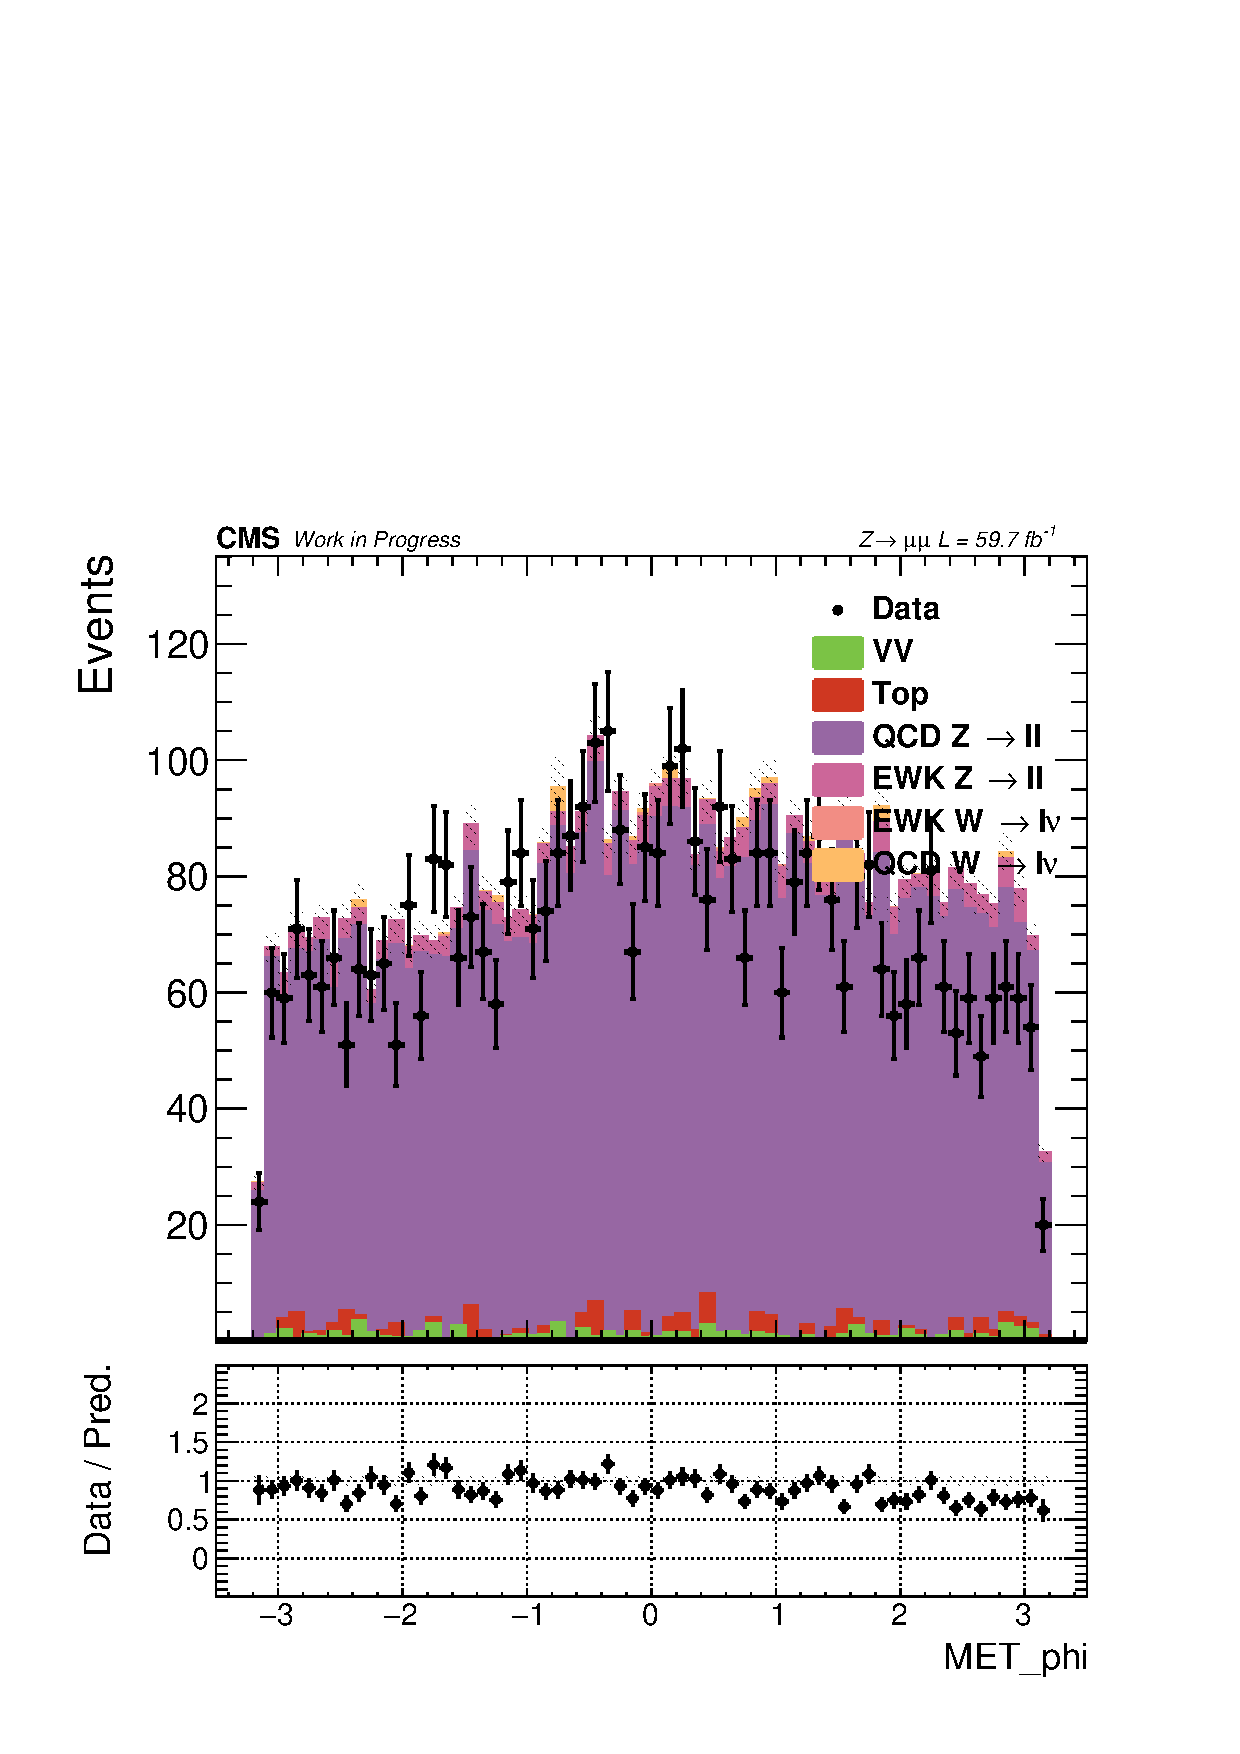
\includegraphics[width=0.49\textwidth]{Control_Regions/Zmumu_noHEM/MetNoMu_phi_Zmumu_MTR_2018.pdf}
    }
    \subfigure[$\phi_{j1}$ - MTR]{
    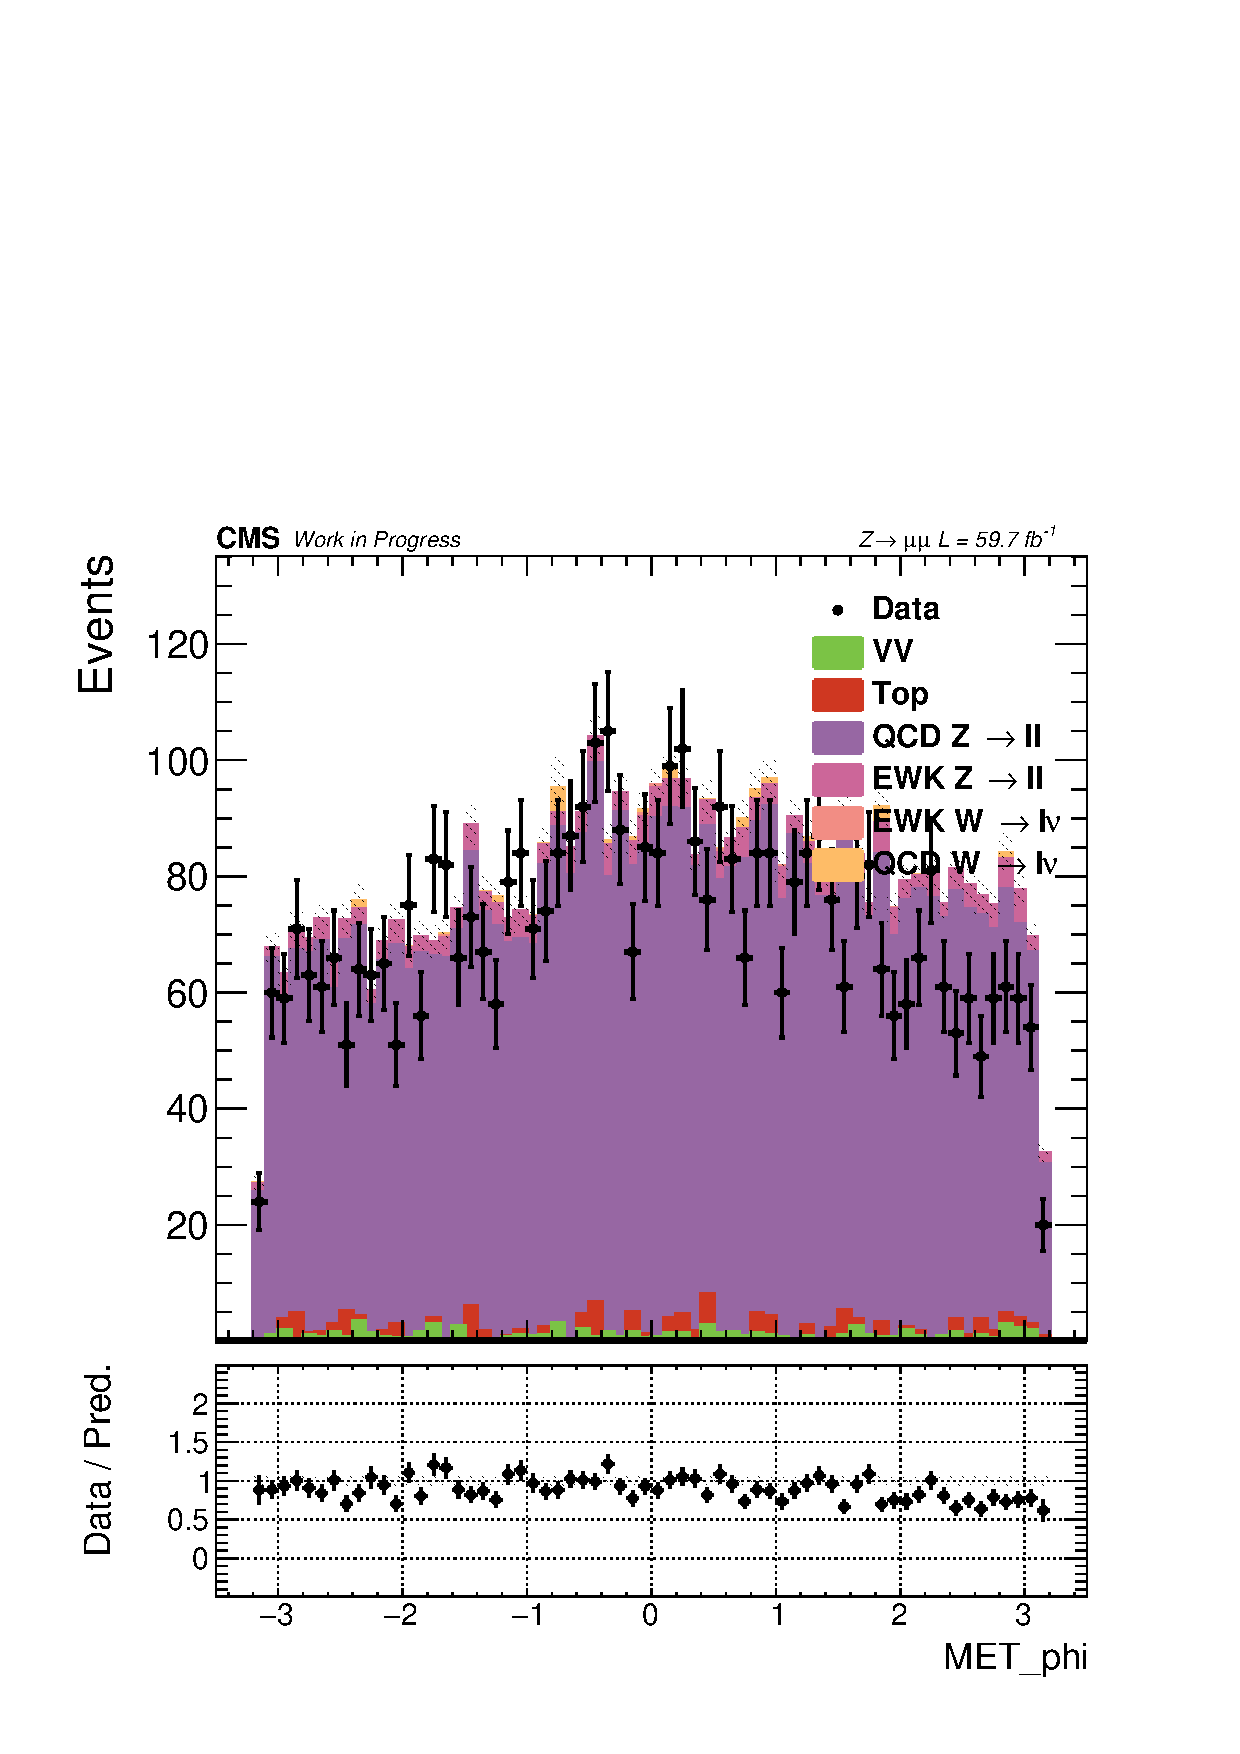
\includegraphics[width=0.49\textwidth]{Control_Regions/Zmumu_noHEM/MetNoMu_phi_Zmumu_MTR_2018.pdf}
    }\\
    \subfigure[$E_{T,miss}$ - VTR]{
    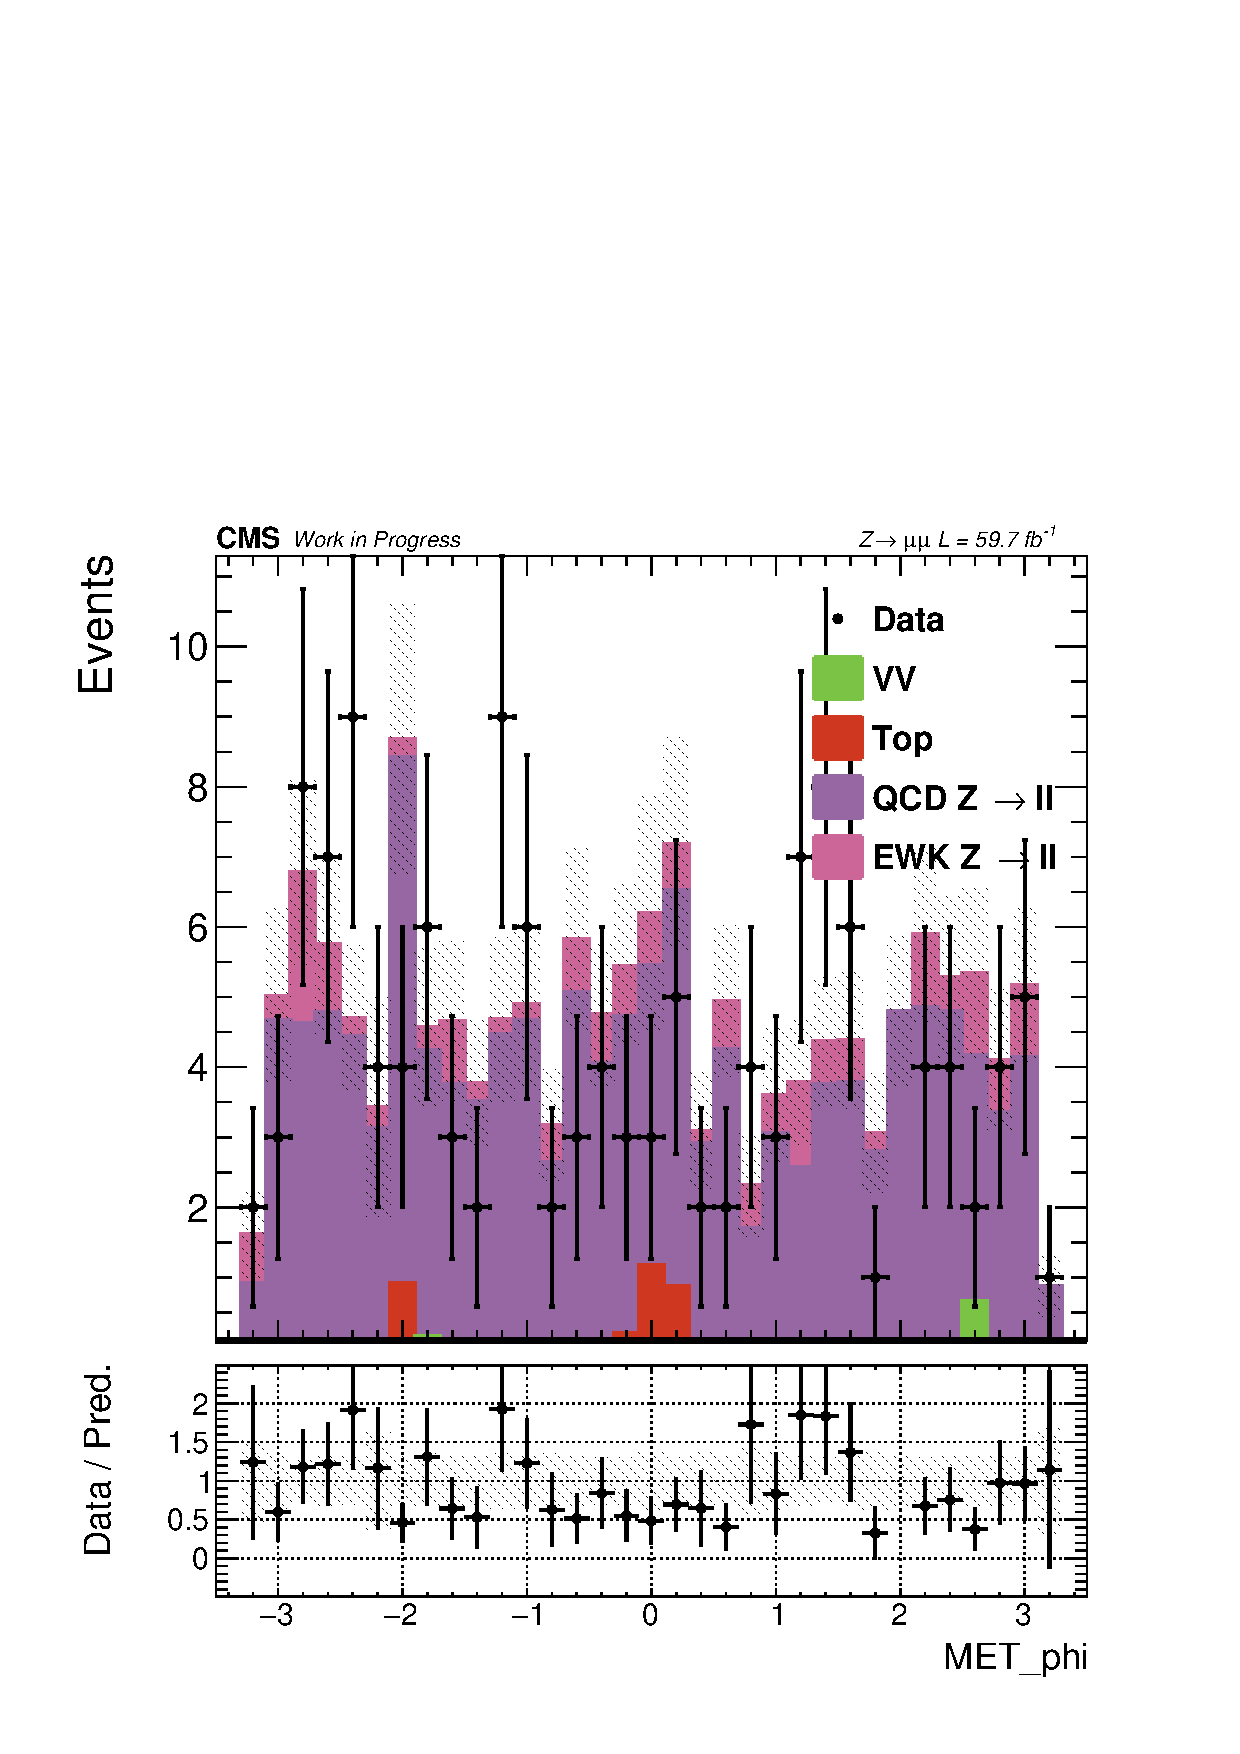
\includegraphics[width=0.49\textwidth]{Control_Regions/Zmumu_noHEM/MetNoMu_phi_Zmumu_VTR_2018.pdf}
    }
    \subfigure[$\phi_{j1}$ - VTR]{
    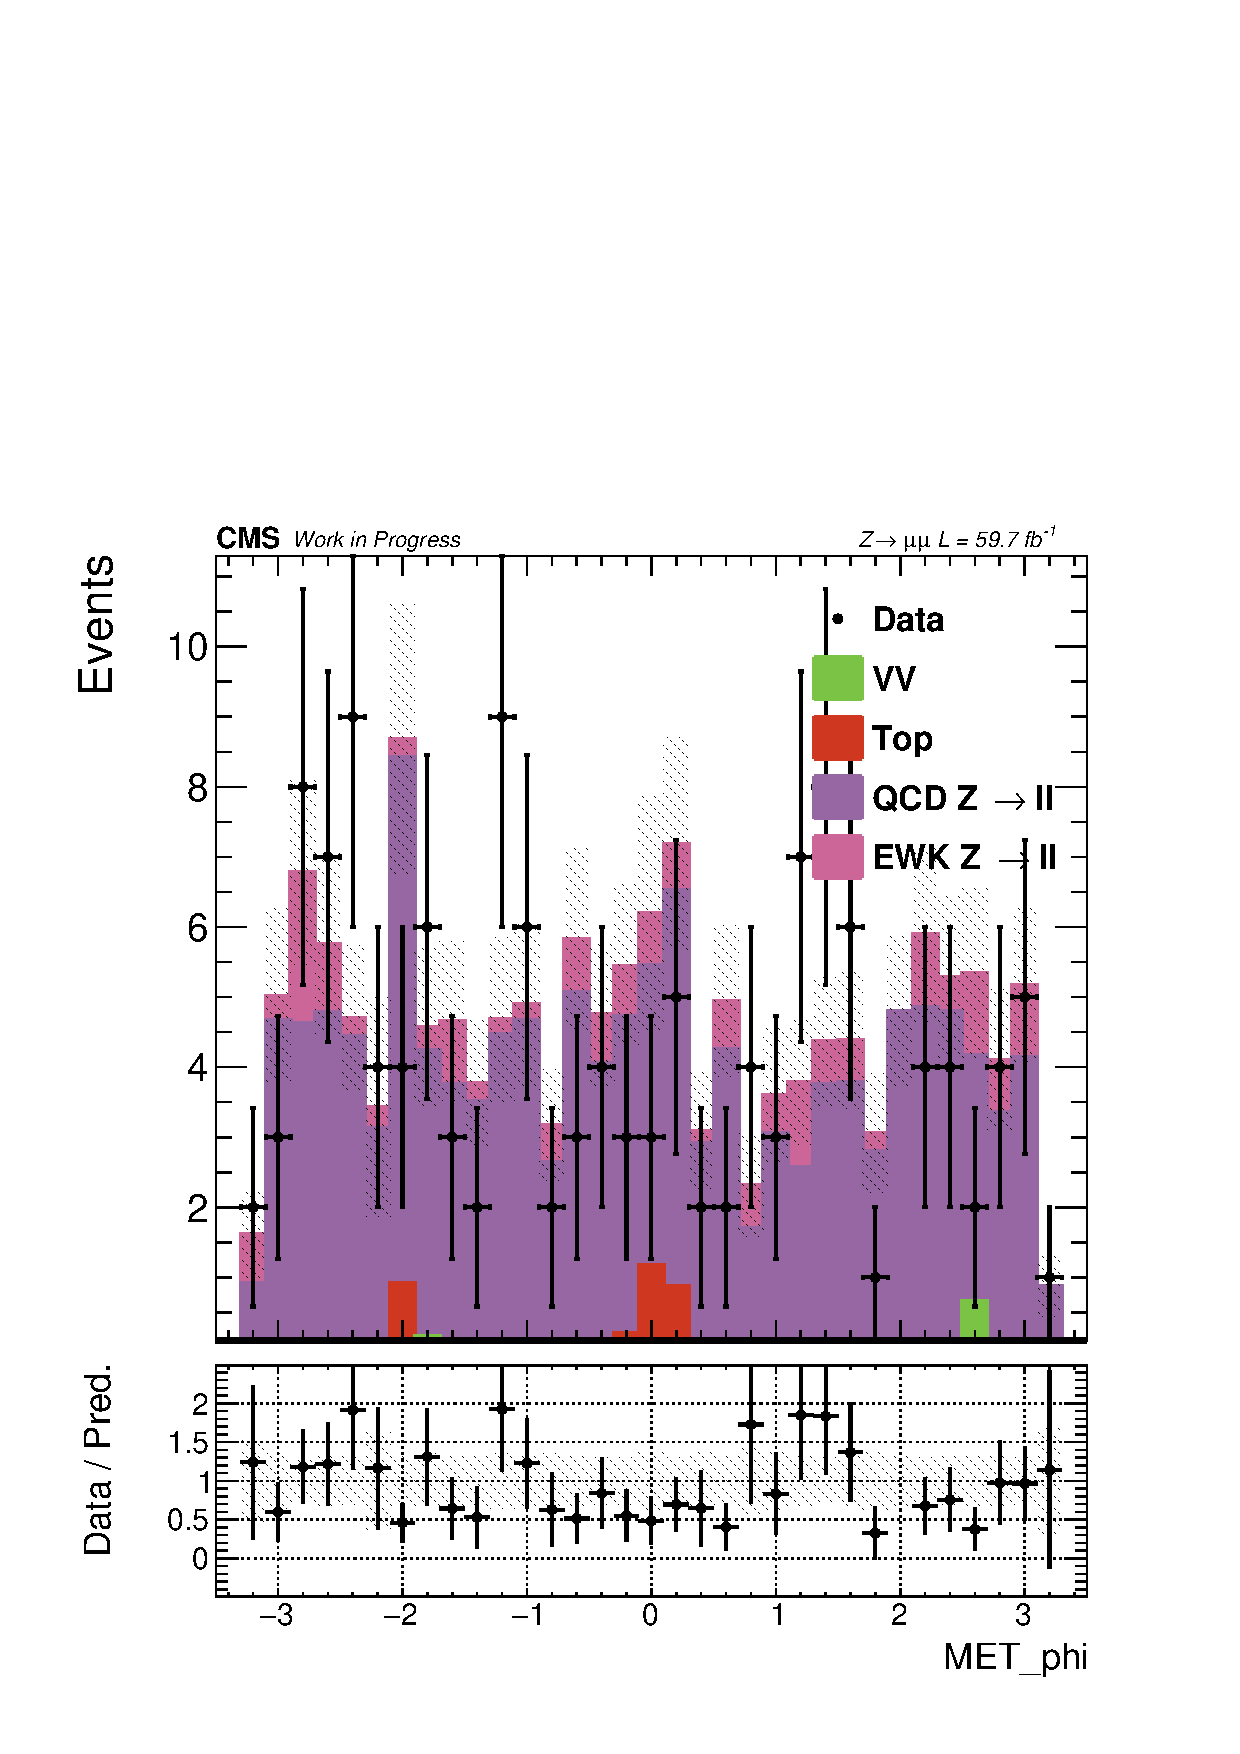
\includegraphics[width=0.49\textwidth]{Control_Regions/Zmumu_noHEM/MetNoMu_phi_Zmumu_VTR_2018.pdf}
    }
  \caption{Distributions of $E_{T,miss}$ (left) and $\phi_{j1}$ (right) variables in the double muon CR showing the absence of effects related to the HEM. Both MTR (top) and (bottom) categories are presented.}
  \label{fig:Zmumu_noHEM}
\end{figure}